\chapter{Modélisation d'un drone convertible : DarkO}
\minitoc
\label{chap:model}

\section{Modèle du drone DarkO}
\label{sec:model}
DarkO est un drone conçu et développé à l'École Nationale de l'Aviation Civile (ENAC) de Toulouse (France), est un exemple clair de drone convertible avec une architecture dite \textit{tailsitter}.
DarkO est assemblé à partir de plusieurs pièces d'Onyx imprimées en 3D (un matériau très robuste composé de fibres de carbone omnidirectionnelles). Toutes les pièces sont emboîtées sur un seul axe, de sorte que le drone puisse facilement être démonté pour remplacer des pièces ou accéder à l'électronique embarquée. 

L'autopilote embarqué est une carte Apogee~\footnote{\url{https://wiki.paparazziuav.org/wiki/Apogee/v1.00}} fabriquée à l'ENAC, voir Fig. \ref{fig:apogee}. 


\begin{figure}[ht]
    \centering
        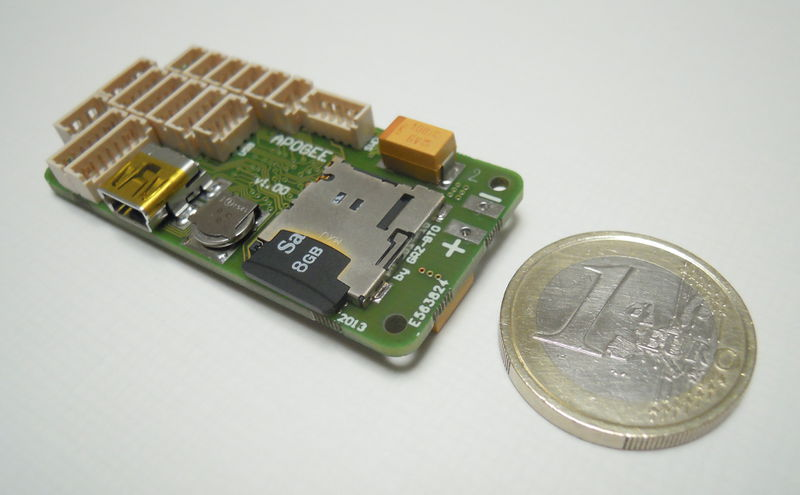
\includegraphics[width=0.8\columnwidth]{figures/800px-Apogee_v100_top_1E.jpeg}
        \caption{Vue de dessus d'un autopilote Apogee v1.00.}
        \label{fig:apogee}
\end{figure}

L'autopilote offre la possibilité d'enregistrer les données de bord sur une carte mémoire SD, à la fréquence de contrôle de 500 Hz, ce qui permet un post-traitement efficace des données acquises. Le protocole de communication utilisé entre l'autopilote et les contrôleurs électroniques de vitesse (ESC) est le Dshot 600. Les ESC sont des AIKON AK32 35A \todo{trouver un synonyme} flasher avec un firmware AM32. La communication sol-bord est réalisée via un canal bidirectionnel basé sur des modules XBee-PRO S1.

\nomenclature[]{\(ESC\)}{Contrôleurs électroniques de vitesse (\textit{Electronic Speed Controller})}

\begin{figure}[ht]
    \centering
    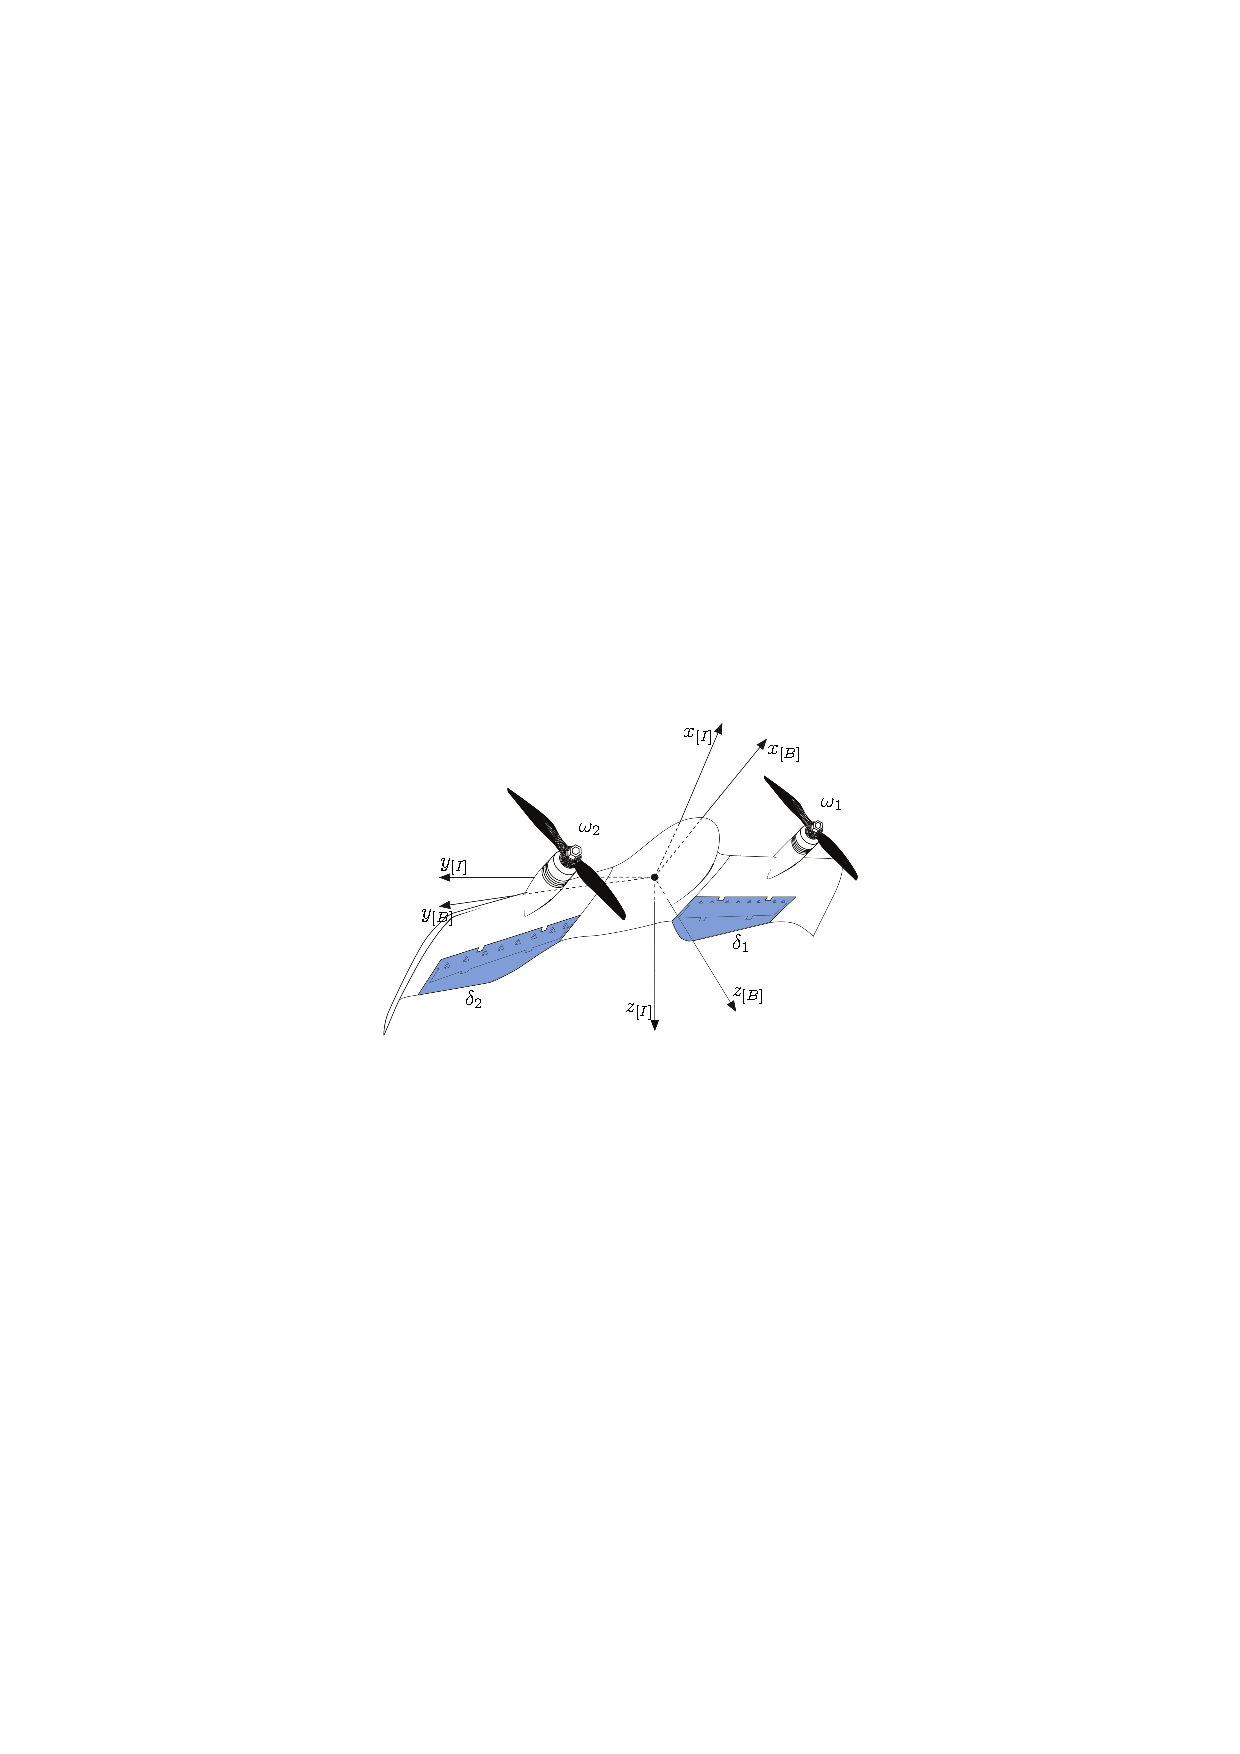
\includegraphics[width=1\columnwidth]{figures/darko.pdf}
    \caption{Repère de référence de DarkO avec une représentation schématique des actionneurs.}
    \label{fig:darko2}
\end{figure}

Les actionneurs de DarkO peuvent être décomposé en deux catégories. La première est composée de deux hélices (T-Motor T5147) placées symétriquement à l'avant de l'aile (illustrées en \textbf{noir} dans la Fig. \ref{fig:darko2}) alimentées par deux moteurs électriques (T-Motor F30 2300kv) générant une traction selon l'axe $x_{b}$. La seconde catégorie est relative aux actionneurs aérodynamiques ainsi le drone possède deux élevons, placés à l'arrière de l'aile (illustrés en \textcolor{cyan}{bleu} dans la Fig. \ref{fig:darko2}), agissant en tant que surfaces de contrôle. Les élevons génèrent des forces et des moments en modifiant leurs incidences relativement au flux d'air dans lequel ils sont placé. Ce flux d'air peut être généré par le vent relatif (liée à la vitesse du drone), le vent extérieur, mais aussi par le souffle des hélices. Les élevons sont commandés par deux servomoteurs MKS DS65K.

La figure \ref{fig:darko2} montre le modèle de DarkO, ainsi qu'un repère de référence inertiel NED (ou repère terrestre) ``$\text{i}$'' lié à la surface de la Terre, et un repère corps `$\text{b}$'' attaché au drone, avec $x_{\text{b}}$ correspondant à l'axe de roulis (l'axe des hélices dans le plan $z_{\text{b}} =0$), $y_{\text{b}}$ l'axe de tangage (la direction des ailes), $z_{\text{b}}$ l'axe de lacet. En utilisant la même notation que dans \cite{lustosa:hal-03035938}, le couple hélice/élévateur gauche et droit sont désignés par les indices $i=1$ (gauche) et $i=2$ (droite). La convention de signe sera définie comme positive pour les positions des élevons $\delta_{1}$, $\delta_{2}$ lorsqu'ils créent un moment à cabrer avec les hélices tournant dans des directions opposées avec des vitesses angulaires $\omega_{1} > 0$ et $\omega_{2} < 0$, respectivement.

\begin{table}[ht]
    \centering
      \begin{tabular}{|l|c|c|}
        \hline
        \multicolumn{1}{|c|}{Paramètres et coefficients} & Valeurs & Unités \\
        \hline
        $m$ (Masse du drone)  & 0.519 & \SI{}{\kilogram} \\
        \hline
        $b$ (Envergure)  & 0.542 & \SI{}{\meter} \\
        \hline
        $c$ (Corde aérodynamique)  & 0.13 & \SI{}{\meter} \\
        \hline
        $\boldsymbol{B}=\diag(b,c,b)$ & $\!\!\diag(0.542, 0.13, 0.542)$ \!\! & \SI{}{\meter}\\
        \hline
        $S$ (Surface de l'aile) & 0.026936 & \SI{}{\square\meter}\\
        \hline
        $S_{\text{wet}}$ (Surface soufflée) & 0.0180 & \SI{}{\square\meter}\\
        \hline
        $S_{\text{p}}$ (Surface de helice) & 0.0127 & \SI{}{\square\meter}\\
        \hline
        $\boldsymbol{J}=\diag(J_{x},J_{y},J_{z})$ & \!\! $\diag(0.0067,0.0012,0.0082)$\!\! & \SI{}{\kilogram\square\meter}\\
        \hline
        $k_{\text{f}}$ (Poussée des hélices) & 1.7800e-8 & \SI{}{\kilogram\meter}\\
        \hline
        $k_{\text{m}}$(Moment des hélices) & 2.1065e-10 & \SI{}{\kilogram\square\meter}\\
        \hline
        $p_{x}$ (Position en $x$ des hélices) & 0.065 & \SI{}{\meter}\\
        \hline
        $p_{y}$ (Position en $y$  des hélices) & 0.162 & \SI{}{\meter}\\
        \hline
        $a_{y}$ (Position en $y$ de la portance) & 0.1504 & \SI{}{\meter}\\
        \hline
        $\xi_{\text{f}}$ (Portance des élevons) & 0.2 & --\\
        \hline
        $\xi_{\text{m}}$ (Moment des élevons) & 1.4 & --\\
        \hline
        $\rho$ (Densité de l'air) & 1.225 & \SI{}{\kilogram\per\cubic\meter}\\
        \hline
        $C_{\text{d}}$ (Trainé) & 0.1644 & --\\
        \hline
        $C_{y}$ (Lateral) & 0 & --\\
        \hline
         $C_{\ell}$ (Portance) & 5.4001 & --\\
        \hline
        $\Delta_{\text{r}}$ (Centrage du drone) & -0.0145 & \SI{}{\meter}\\
        \hline
      \end{tabular}
      \caption{\label{tab:pars} Paramètres numériques identifiés du modèle DarkO.}
\end{table}

\subsection{Modèle non-linéaire complet}

En exploitant la modélisation présentée dans \cite{lustosa:hal-03035938} et \cite{olszaneckibarth:hal-02542982}, un modèle précis de la dynamique de DarkO décrit la position $\boldsymbol{p} \in \real^3$ du centre de gravité et sa vitesse $\boldsymbol{v} = \dot{\boldsymbol{p}} \in \real^3$, en plus de son orientation, bien représentée par un quaternion $\boldsymbol{q} \in {\mathbb S}^3:=\{ \boldsymbol{q} \in \real^4 : |\boldsymbol{q}| = 1\}$ et de sa vitesse angulaire $\boldsymbol{\omega}_{\text{b}}$ représentée dans le repère du corps, qui satisfait $boldsymbol{\dot q} = \frac{1}{2}\boldsymbol{q} \otimes \smallmat{0 \\ \boldsymbol{\omega}_{{\text{b}}}}$, où $\otimes$ représente le produit de Hamilton (voir \cite{lustosa:hal-03035938,olszaneckibarth:hal-02542982} ou le tutoriel \cite{hamel_minhduc} pour plus de détails). En choisissant l'état global comme $\boldsymbol{x}:=(\boldsymbol{p},~ \boldsymbol{v},~ \boldsymbol{q},~ \boldsymbol{\omega}_{\text{b}})$, le modèle mathématique dérivé dans \cite{lustosa:hal-03035938}, dépendent d'un ensemble de paramètres énumérés dans le tableau \ref{tab:pars}, où nous indiquons également la valeur obtenue à partir d'une identification du système \cite{sansou:stage}. Le modèle dynamique peut être écrit comme ci-dessous :

\begin{subequations}\label{eq:dyna_orig}
    \begin{empheq}[left=\empheqlbrace]{alignat=2}
          % \boldsymbol{\dot p} & &= & \boldsymbol{v} \label{eq:dyna1}\\
          m\boldsymbol{\dot v} &&=& - m\boldsymbol{g} +  \boldsymbol{R}(\boldsymbol{q})\boldsymbol{F}_{\text{b}},\\
          \label{eq:dyna_orig_b}
          \boldsymbol{J} \boldsymbol{\dot \omega_{\text{b}}} &&= &  - \skewsym{\boldsymbol{\omega}_{\text{b}}}\boldsymbol{J}\boldsymbol{\omega}_{\text{b}} + \boldsymbol{M}_{\text{b}},
    \end{empheq}
  \end{subequations}
  où $\boldsymbol{g}:=\smallmat{0 & 0& 9.81}^\top$ désigne le vecteur de gravité, $m\in \real$ est la masse, $\boldsymbol{J}\in \real^{3\times 3}$ est le moment d'inertie diagonal (voir Tableau~\ref{tab:pars}) et en partitionnant le quaternion $\boldsymbol{q} \in {\mathbb S}^3$ comme $\boldsymbol{q} := \left[ \eta ~ \boldsymbol{\epsilon}^\top \right]^\top$, la matrice de rotation correspondante est $\boldsymbol{R}(\boldsymbol{q}) \in SO(3): = \{\boldsymbol{R}\in \real^{3\times 3}: \; \boldsymbol{R}^\top \boldsymbol{R} = \mathbb{I}_{3}, \det (\boldsymbol{R})=1\}$ est défini comme (voir \cite{hamel_minhduc})
\begin{align}
    \label{eq:matrix_rot}
    \boldsymbol{R}(\boldsymbol{q}) := \mathbb{I}_{3} +2\eta \skewsym{\boldsymbol{\epsilon}} + 2\skewsym{\boldsymbol{\epsilon}}^{2}.
\end{align}


D'après \cite{lustosa:hal-03035938} le vecteur de force et de moment $\boldsymbol{F}_{\text{b}}$ et $\boldsymbol{M}_{\text{b}}$ dans \eqref{eq:dyna_orig} dépendent  (i) de l'état du système $\boldsymbol{x}$, (ii) de la perturbation $\boldsymbol{w} \in \real^3$, représentant la vitesse du vent dans le référentiel inertiel, et (iii) de la commande des actionneurs (voir Figure~\ref{fig:darko2}), comprenant la vitesse de rotation des deux hélices $\omega_1, \omega_2 \in \real$ et la déflexion des élevons $\delta_1, \delta_2\in \real$.
Considérons d'abord l'effet des commandes des actionneurs. Chaque hélice génère une poussée $\boldsymbol{T}_i$ orienté dans la direction $x$ du repère corps et un moment $\boldsymbol{N}_i$ selon le même axe :
\begin{align}
\label{eq:thrust}
\boldsymbol{T}_{i} \!:=\! \begin{bmatrix} \tau_{i} \\ 0 \\ 0 \end{bmatrix} \!:=\!
\begin{bmatrix} k_{\text{f}}\omega_{i}^{2} \\ 0 \\ 0 \end{bmatrix}\! , \;
\boldsymbol{N}_{i} \!:=\! (-1)^{i}  \frac{k_{\text{m}} }{k_{\text{f}}}\boldsymbol{T}_{i}, \quad i=1,2 .
\end{align} 

La position de chaque élevon $\delta_i \in \real$ est assignée par un servomoteur qui impose un niveau d'efficacité (en termes de déviation du courant d'air) quantifié par deux matrices antisymétriques :
\begin{align}
\label{eq:elevons_efficiency}
    \boldsymbol{\Delta}^{\text{f}}_{i} \!:=\! \begin{bmatrix} 0 & 0 & \xi_{\text{f}}\delta_{i} \\ 0 & 0 & 0 \\ -\xi_{\text{f}}\delta_{i} & 0 & 0 \end{bmatrix}\! ,\;
    \boldsymbol{\Delta}^{\text{m}}_{i} \!:=\! \begin{bmatrix} 0 & 0 & \xi_{\text{m}}\delta_{i} \\ 0 & 0 & 0 \\ -\xi_{\text{m}}\delta_{i} & 0 & 0 \end{bmatrix} \!, 
\end{align}
$i=1,2$. Les paramètres constants $k_{\text{f}}$, $k_{\text{m}}$, $\xi_{\text{f}}$, $\xi_{\text{m}}$ apparaissant dans \eqref{eq:thrust} et \eqref{eq:elevons_efficiency} sont listés dans la Table~\ref{tab:pars}.\\
Avec les quantités ci-dessus, nous pouvons réarranger la dynamique donnée dans le tableau suivant \cite[eqns (97),~(98)]{lustosa:hal-03035938} (voir aussi \cite{sansou:stage}) et exprimer $\boldsymbol{F}_{\text{b}}$ et $\boldsymbol{M}_{\text{b}}$ dans \eqref{eq:dyna_orig} comme
%
\begin{align}
\nonumber
    \boldsymbol{F}_{\text{b}} :={}&  \boldsymbol{T}_{1} + \boldsymbol{T}_{2} + \frac{S_{\text{wet}}}{4S_{\text{p}}} \boldsymbol{\Phi}^{\text{(fv)}} \Big( (\boldsymbol{\Delta}^{\text{f}}_1 - \mathbb{I}_{3} ) \boldsymbol{T}_{1} + ( \boldsymbol{\Delta}^{\text{f}}_2 - \mathbb{I}_{3}) \boldsymbol{T}_{2}\Big) \\ 
     \label{eq:Fb}
    &+ \frac{1}{4} \rho S  \boldsymbol{\Phi}^{\text{(fv)}} \Big(\boldsymbol{\Delta}^{\text{f}}_1+ \boldsymbol{\Delta}^{\text{f}}_2 - 2 \mathbb{I}_{3} \Big) \lVert \boldsymbol{v_{\text{b}}} \rVert \boldsymbol{v_{\text{b}}}\\
    \nonumber
    &+ \frac{1}{4} \rho S \boldsymbol{\Phi}^{\text{(mv)}} \Big(\boldsymbol{\Delta}^{\text{f}}_1 + \boldsymbol{\Delta}^{\text{f}}_2 - 2\mathbb{I}_{3}\Big) \boldsymbol{B} \lVert \boldsymbol{v_{\text{b}}} \rVert  \boldsymbol{\omega}_{\text{b}}, 
\end{align}
\begin{align} 
\label{eq:Mb}
 \boldsymbol{M}_{\text{b}} :&=\boldsymbol{N}_{1} + \boldsymbol{N}_{2} + \skewsym{\smallm{p_x\\ p_y\\ 0}} \boldsymbol{T}_{1} + \skewsym{\smallm{p_x\\ - p_y\\ 0}} \boldsymbol{T}_{2}\\
    \nonumber
  &- \frac{S_{\text{wet}}}{4S_{\text{p}}} \bigg( \boldsymbol{B} \boldsymbol{\Phi}^{\text{(mv)}} (\boldsymbol{\Delta}^{\text{m}}_1- \mathbb{I}_{3} ) + \skewsym{\smallm{0 \\ a_y \\ 0}} \boldsymbol{\Phi}^{\text{(fv)}} (\boldsymbol{\Delta}^{\text{m}}_1 +\mathbb{I}_{3} ) \bigg) \boldsymbol{T}_{1} \\
    \nonumber
  & - \frac{S_{\text{wet}}}{4S_{\text{p}}} \bigg( \boldsymbol{B} \boldsymbol{\Phi}^{\text{(mv)}} (\boldsymbol{\Delta}^{\text{m}}_2 - \mathbb{I}_{3} ) +  \skewsym{\smallm{0 \\ - a_y \\ 0}} \boldsymbol{\Phi}^{\text{(fv)}} (\boldsymbol{\Delta}^{\text{m}}_2 + \mathbb{I}_{3}) \bigg) \boldsymbol{T}_{2} \\
    \nonumber
  & + \frac{1}{4} \rho S  \bigg( \Big(\skewsym{\smallm{0 \\ a_y \\ 0}} \!\!\! \boldsymbol{\Phi}^{\text{(fv)}}  + \boldsymbol{B} \boldsymbol{\Phi}^{\text{(mv)}} \Big) \boldsymbol{\Delta}^{\text{m}}_1 \\
    \nonumber
  &  + \Big( \skewsym{\smallm{0 \\ - a_y \\ 0}} \!\!\! \boldsymbol{\Phi}^{\text{(fv)}} + \boldsymbol{B} \boldsymbol{\Phi}^{\text{(mv)}}  \Big) \boldsymbol{\Delta}^{\text{m}}_2 - 2 \boldsymbol{B} \boldsymbol{\Phi}^{\text{(mv)}}  \bigg) \lVert \boldsymbol{v_{\text{b}}} \rVert \boldsymbol{v_{\text{b}}} \\
    \nonumber
  & +\frac{1}{4} \rho S \bigg(\!\! \Big(\!\! \skewsym{\!\smallm{0 \\ a_y \\ 0}\!}\!\!\! \boldsymbol{\Phi}^{\text{(mv)}} \! + \! \boldsymbol{B} \boldsymbol{\Phi}^{\text{(m$\omega$)}} \Big) \boldsymbol{\Delta}^{\text{m}}_1 \\
    \nonumber
  & +  \Big(\!\! \skewsym{\!\smallm{0 \\ - a_y \\ 0}\!} \!\!\! \boldsymbol{\Phi}^{\text{(mv)}} \! + \! \boldsymbol{B} \boldsymbol{\Phi}^{\text{(m$\omega$)}}  \Big) \boldsymbol{\Delta}^{\text{m}}_2 - 2 \boldsymbol{B} \boldsymbol{\Phi}^{\text{(m$\omega$)}}\!  \bigg)\!  \boldsymbol{B}  \lVert \boldsymbol{v_{\text{b}}} \rVert  \boldsymbol{\omega}_{\text{b}} ,
\end{align}
où $\boldsymbol{v}_{\text{b}} := \boldsymbol{R}^\top(\boldsymbol{q}) (\boldsymbol{v}-\boldsymbol{w})$ représente la vitesse de l'air vu par le drone exprimé dans le repère du corps. Dans \cite{lustosa:hal-03035938}, la valeur $\lVert \boldsymbol{v_{\text{b}}} \rVert$ apparaissatn dans les expressions de  $\boldsymbol{F}_{\text{b}}$ et $\boldsymbol{M}_{\text{b}}$ est remplacé par la valeur $\eta = \sqrt{\lVert \boldsymbol{v_{\text{b}}} \rVert^{2} + \mu c^{2} \lVert \boldsymbol{\omega}_{\text{b}} \rVert^{2}}$, avec $\mu \in \real$ étant un paramètre lié à l'identification du modèle, mais dans le cas de DarkO \cite{sansou:stage}, l'identification fournit $\mu = 0$, c'est pourquoi nous présentons ici une description simplifiée. La matrice des coefficients aérodynamiques constants 
$\boldsymbol{\Phi}:= \begin{bmatrix} \boldsymbol{\Phi}^{\text{(fv)}} & {\boldsymbol{\Phi}^{\text{(mv)}}}^\top \\ \boldsymbol{\Phi}^{\text{(mv)}} & \boldsymbol{\Phi}^{\text{(m$\omega$)}} \end{bmatrix} \in \real^{6 \times 6}$, est défini dans \cite[eqs. (6)--(9)]{olszaneckibarth:hal-02542982} comme $ \boldsymbol{\Phi}^{\text{(fv)}} \!:=\! \diag(C_{\text{d}},C_{y}, C_{\ell})$ et
\begin{align*}
&\left[ \begin{array}{c|c}
    \boldsymbol{\Phi}^{\text{(mv)}}  &  \boldsymbol{\Phi}^{\text{(m$\omega$)}} 
\end{array}\right] :=\\ 
&\left[ \begin{array}{ccc|ccc}
    0 & 0 & 0    &                                          0.1396 & 0 & 0.0573 \\
    0 & 0 & \!\!\!\!\! -\frac{\Delta_{\text{r}}}{c}C_{\ell} &    0 &  0.6358  & 0 \\
    0 & 0 & 0 &     0.0405 & 0 & 0.0019 
\end{array}\right],
\end{align*}
les valeurs numériques des constantes figurant dans le tableau \ref{tab:pars} (ces valeurs numériques n'ont pas été indiquées dans \cite{lustosa:hal-03035938} et \cite{olszaneckibarth:hal-02542982} et sont données ici pour permettre de reproduire les résultats de nos simulations). 


\subsection{Modèle non linéaire simplifiée à basse vitesse}

Comme nous allons nous intéresser au maintien du drone en stationnaire, où la vitesse du drone est faible, nous pouvons simplifier la dynamique \eqref{eq:dyna_orig} en négligeant les effets aérodynamique quadratique dû à la vitesse $\boldsymbol{v_{\text{b}}}$ et à la vitesse angulaire $\boldsymbol{\omega}_{\text{b}}$ dans \eqref{eq:Fb} et \eqref{eq:Mb}. 
Nous définissons le vecteur de commande :
\begin{align}
\label{eq:vector_u}
    \boldsymbol{u} := \begin{bmatrix}\tau_{1}  \!&\! \tau_{2}  \!&\! \delta_{1} \!&\! \delta_{2} \end{bmatrix}^\top,
\end{align}
qui permet d'obtenir le modèle basse vitesse comportant majeur les effets non linéaires du vent  
\begin{subequations}\label{eq:dyna_simp}
    \begin{alignat}{3}
    &\boldsymbol{\dot p} = \boldsymbol{v}, \label{eq:dyna1}\\
       & m\boldsymbol{\dot v} =\! \shortminus m\boldsymbol{g} \!+ \! \boldsymbol{R} (\boldsymbol{q}) \!\!\left( \! \boldsymbol{M}_{\text{f}}(\boldsymbol{u}) \! + \! \boldsymbol{D}_{\text{f}}(\boldsymbol{u}) \| \boldsymbol{w} \| \boldsymbol{R}^\top \!(\boldsymbol{q}) (\boldsymbol{v} \! \shortminus \! \boldsymbol{w}) \! \right)\!,\!\! \label{eq:dyna2}\\
        &\boldsymbol{\dot q} = \frac{1}{2}\boldsymbol{q} \otimes \smallmat{0 \\ \boldsymbol{\omega}_{\text{b}}}, \label{eq:dyna3}\\
        &\boldsymbol{J} \boldsymbol{\dot \omega}_{\text{b}} = \shortminus \skewsym{\boldsymbol{\omega}_{\text{b}}}\boldsymbol{J}\boldsymbol{\omega}_{\text{b}}\! + \boldsymbol{M}_{\text{m}}(\boldsymbol{u})\! + \boldsymbol{D}_{\text{m}} (\boldsymbol{u}) \lVert \boldsymbol{w} \rVert \boldsymbol{R}^\top(\boldsymbol{q}) (\boldsymbol{v}-\boldsymbol{w}), \label{eq:dyna4}
    \end{alignat}
\end{subequations}
où les vecteurs $\boldsymbol{M}_{\text{f}}(\boldsymbol{u})$ et $ \boldsymbol{M}_{\text{m}}(\boldsymbol{u})$, et les matrices $\boldsymbol{D}_{\text{f}}(\boldsymbol{u})$ et $\boldsymbol{D}_{\text{m}} (\boldsymbol{u})$ proviennent de l'annulation des termes dépendant de la vitesse angulaire dans l'équation \eqref{eq:Fb} et \eqref{eq:Mb}. Ils peuvent etre développer en 
\begin{align}
\label{eq:Mf}
    &\boldsymbol{M}_{\text{f}}(\boldsymbol{u}) :=  \boldsymbol{T}_{1} \!+\! \boldsymbol{T}_{2} \!+\! \frac{S_{\text{wet}}}{4S_{\text{p}}} \boldsymbol{\Phi}^{\text{(fv)}} \Big( (\boldsymbol{\Delta}^{\text{f}}_1 \shortminus \mathbb{I}_{3} ) \boldsymbol{T}_{1} + ( \boldsymbol{\Delta}^{\text{f}}_2 \shortminus \mathbb{I}_{3}) \boldsymbol{T}_{2}\Big) \nonumber\\
& \hspace*{1.2cm} =\begin{bmatrix} \left(1-\frac{S_{\text{wet}}}{4S_{\text{p}}} C_{\text{d}}\right) (\tau_{1} + \tau_{2}) \\  0  \\ -\frac{S_{\text{wet}}}{4S_{\text{p}}}C_{\ell}\xi_{\text{f}} \left(\delta_{1}\tau_{1} + \delta_{2}\tau_{2}\right) \end{bmatrix}  \\
\nonumber
 & \boldsymbol{M}_{\text{m}}(\boldsymbol{u}) := \boldsymbol{N}_{1} + \boldsymbol{N}_{2} + \skewsym{\smallm{p_x\\ p_y\\ 0}} \boldsymbol{T}_{1} + \skewsym{\smallm{p_x\\ -p_y\\ 0}} \boldsymbol{T}_{2}\\
 \nonumber
   &\qquad \shortminus \frac{S_{\text{wet}}}{4S_{\text{p}}}\! \bigg( \boldsymbol{B} \boldsymbol{\Phi}^{\text{(mv)}} (\boldsymbol{\Delta}^{\text{m}}_1- \mathbb{I}_{3} ) \! + \! \skewsym{\smallm{0 \\ a_y \\ 0}} \!\! \boldsymbol{\Phi}^{\text{(fv)}} (\mathbb{I}_{3} + \boldsymbol{\Delta}^{\text{m}}_1 ) \bigg) \boldsymbol{T}_{1} \\
   \nonumber
   &\qquad \shortminus \frac{S_{\text{wet}}}{4S_{\text{p}}} \!\bigg( \boldsymbol{B} \boldsymbol{\Phi}^{\text{(mv)}} (\boldsymbol{\Delta}^{\text{m}}_2 - \mathbb{I}_{3} ) \! + \! \skewsym{\smallm{0 \\ \!\shortminus a_y \!\\ 0}} \!\! \boldsymbol{\Phi}^{\text{(fv)}} (\mathbb{I}_{3} + \boldsymbol{\Delta}^{\text{m}}_2 ) \bigg) \boldsymbol{T}_{2} \\
   \label{eq:Mm}
   & \hspace*{1.2cm} =\begin{bmatrix} \frac{k_{\text{m}} }{k_{\text{f}}}(\tau_{1} - \tau_{2}) + \frac{S_{\text{wet}}}{4S_{\text{p}}}a_{y}C_{\ell}\xi_{\text{f}}(\delta_{1}\tau_{1} - \delta_{2}\tau_{2}) \\
   \frac{S_{\text{wet}}}{4S_{\text{p}}} \Delta_{\text{r}}C_{\ell}\xi_{\text{m}}(\delta_{1}\tau_{1} + \delta_{2}\tau_{2}) \\
   \left(p_{y}+\frac{S_{\text{wet}}}{4S_{\text{p}}} a_{y} C_{\text{d}}\right)(\tau_{1} - \tau_{2})
   \end{bmatrix} \\
    \label{eq:df}
             &\boldsymbol{D}_{\text{f}}(\boldsymbol{u}) :=  \frac{1}{4} \rho S  \boldsymbol{\Phi}^{\text{(fv)}} \Big( \boldsymbol{\Delta}^{\text{f}}_1+  \boldsymbol{\Delta}^{\text{f}}_2 - 2 \mathbb{I}_{3} \Big)   \\
            &\hspace*{1.1cm} = \frac{1}{4}\rho S  \begin{bmatrix}
                -2C_{\text{d}} & 0 & C_{\text{d}}\xi_{\text{f}}(\delta_{1} +\delta_{2})\\
                0 & 0 & 0\\
                -C_{\ell}\xi_{\text{f}}(\delta_{1} +\delta_{2}) & 0 & -2C_{\ell}
            \end{bmatrix} \nonumber \\
      \label{eq:dm}      
      & \boldsymbol{D}_{\text{m}}(\boldsymbol{u}) := \frac{1}{4} \rho S  \bigg( \Big(\skewsym{\smallm{0 \\ a_y \\ 0}} \!\!\!  \boldsymbol{\Phi}^{\text{(fv)}}  +  \boldsymbol{B}  \boldsymbol{\Phi}^{\text{(mv)}} \Big)  \boldsymbol{\Delta}^{\text{m}}_1  \\
       &\hspace{0.8cm}  + \Big( \skewsym{\smallm{0 \\ -a_y \\ 0}} \!\!\!  \boldsymbol{\Phi}^{\text{(fv)}} +  \boldsymbol{B}  \boldsymbol{\Phi}^{\text{(mv)}}  \Big)  \boldsymbol{\Delta}^{\text{m}}_2 - 2  \boldsymbol{B}  \boldsymbol{\Phi}^{\text{(mv)}}  \bigg) \nonumber \\
       \nonumber
         & \hspace*{1.1cm} = \frac{1}{4}\rho S  \begin{bmatrix}
                \shortminus a_{y}C_{\text{d}}\xi_{\text{m}}(\delta_{1} \!-\! \delta_{2}) \!\! & 0 & 0\\
                \Delta_{\text{r}}C_{\ell}\xi_{\text{m}}(\delta_{1} +\delta_{2})\!\! & 0 & 2\Delta_{\text{r}}C_{\ell}\\
               0 & 0 & \!\! \shortminus a_{y}C_{\ell}\xi_{\text{m}}(\delta_{1} \!-\!\delta_{2})
            \end{bmatrix} 
    \end{align}
où l'on observe l'effet non linéaire d'un vent non nul, qui est non linéaire avec $\boldsymbol{q}$, $\lVert \boldsymbol{v}_{\text{b}} \rVert$ et $\boldsymbol{w}$. Comme dans \cite[eqn. (10)]{olszaneckibarth:hal-02542982} et selon la formule de Diederich, nous obtenons $C_{\ell} = C_{\text{d}} + \frac{\pi AR}{1+\sqrt{1+\left(\frac{AR}{2}\right)^{2}}}$ où $AR = \frac{b^{2}}{S}$ est l'allongement de l'aile.
Nous observons le couplage des actionneurs $\left(\delta_{1}\tau_{1} + \delta_{2}\tau_{2}\right)$  dans les expressions des matrices $\boldsymbol{M}_{\text{f}}(\boldsymbol{u})$ et $\boldsymbol{M}_{\text{m}}(\boldsymbol{u})$.

\section{Identification des paramètres du modèle}
    Les valeurs numériques du tableau \ref{tab:pars} ont été obtenues par une campagne d'identification du modèle \cite{sansou:stage}. En particulier, le coefficient $k_{\text{f}}$ a été identifié à partir de l'équation \eqref{eq:thrust}, qui relie la vitesse de rotation du moteur $\omega_{i}$ à la traction générée, à la vitesse de rotation minimale et maximale et à la constante de temps de la chaîne d'actionnement du moteur. Les éléments diagonaux de l'inertie $\boldsymbol{J}$ ont été mesurés à l'aide d'un système de pendule bifilaire. Cette méthode est largement utilisée dans le domaine des drones \cite{Jardin2007OptimizedMO}, et est basée sur la période d'oscillation autour de chacun des trois axes ($x_{{\text{b}}}$, $y_{text{b}}$, $z_{\text{b}}$) du drone suspendu par deux fils, ce qui forme un pendule de torsion comme le montre la Fig. \ref{fig:BifilarPend}.
    Il est intéressant de noter que la surface soufflée par les hélices représente 67 \% de la surface totale du drone.


    \begin{figure}[ht!]
        \centerline{
        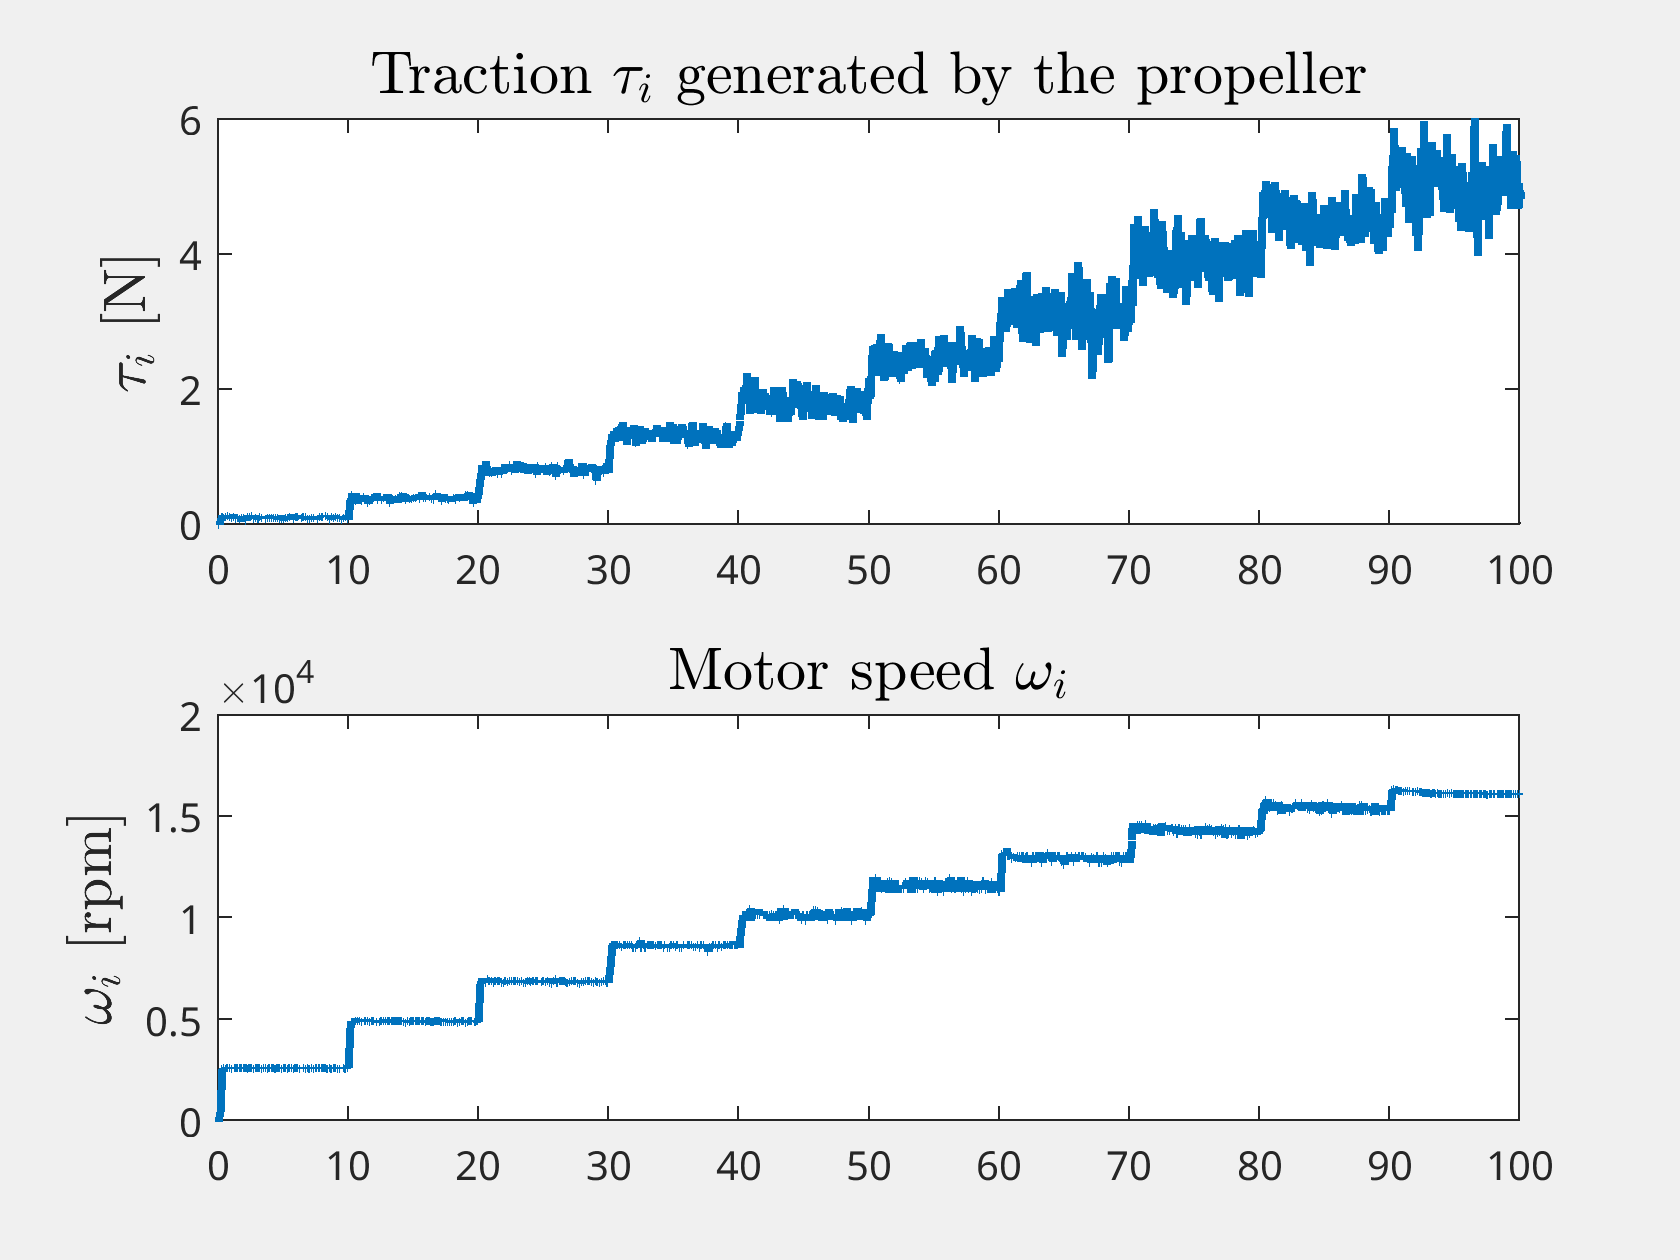
\includegraphics[trim=0cm 0cm 0cm 0cm,clip,width=0.5\columnwidth]{figures/ident_motor March 27 2024 1651.png}}
        \caption{Input-output response of an Esc-Motor-Propeller assembly.}
        \label{IOmot}
    \end{figure}

    \begin{figure}[ht!]
        \centerline{
        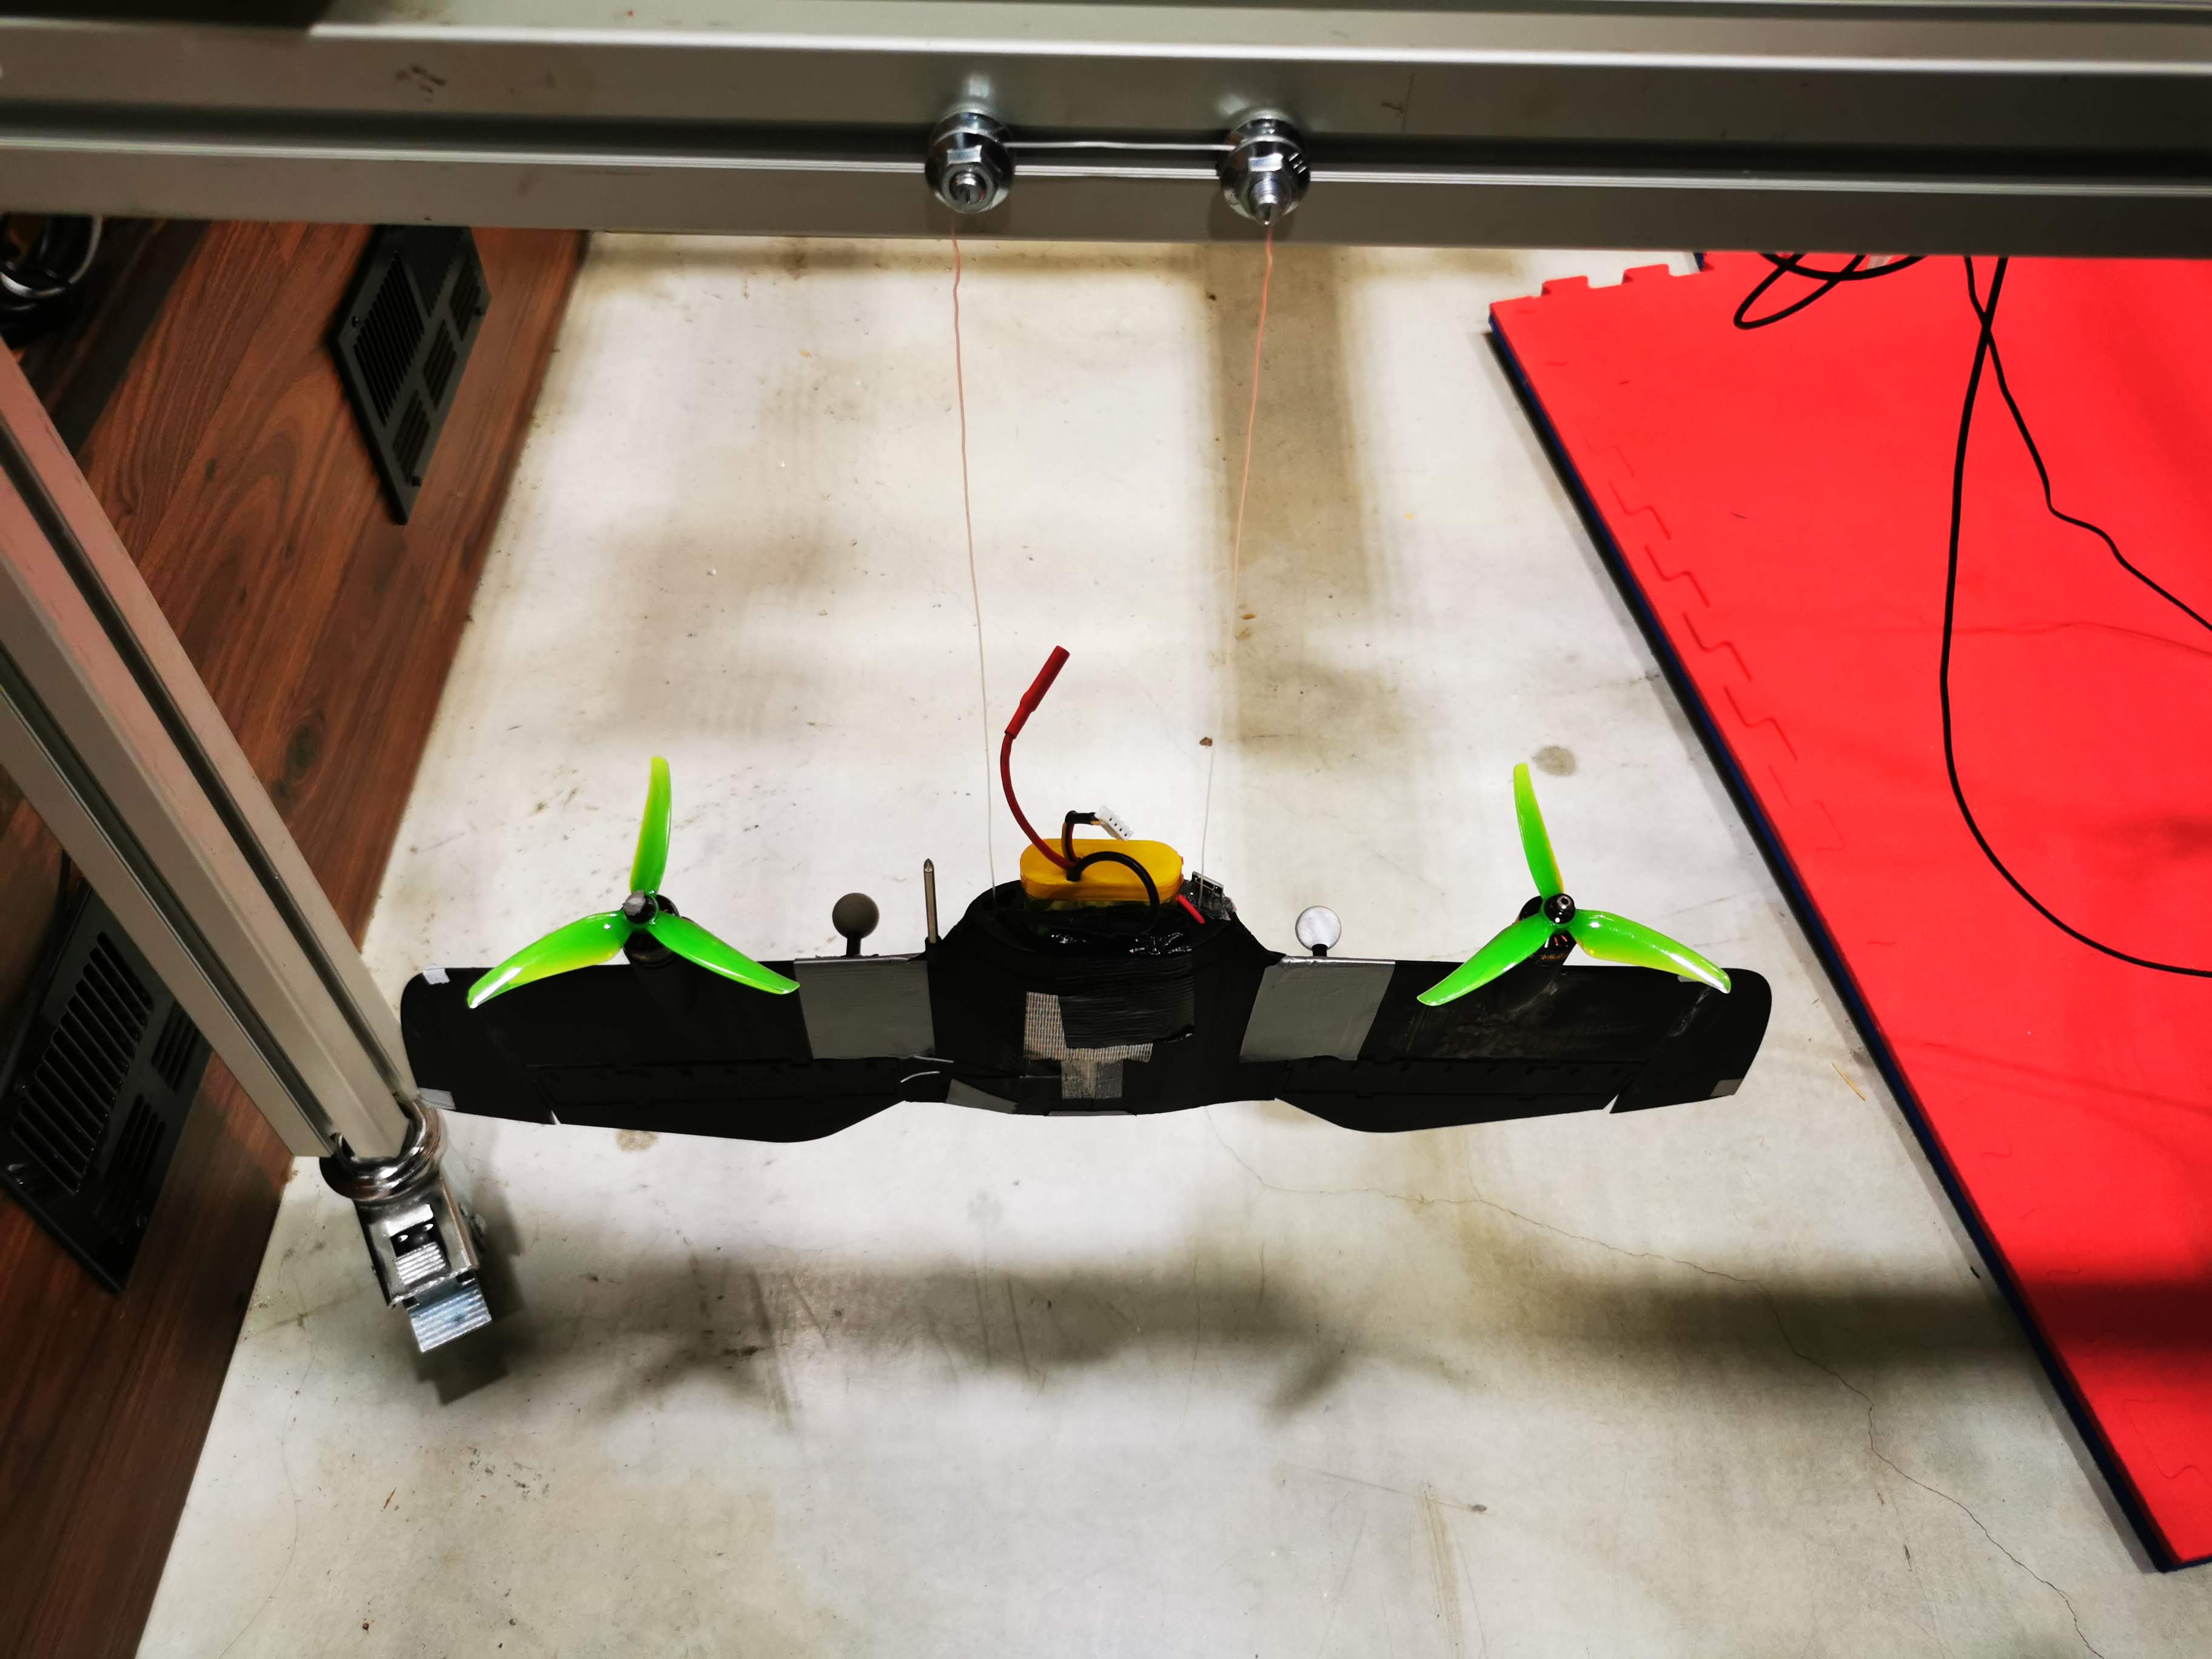
\includegraphics[trim=20cm 15cm 23cm 0cm,clip,width=0.6\columnwidth]{figures/IMG_20230609_085023.jpg}}
        \caption{Bifilar pendulum mounting for the identication of $\boldsymbol{J}$.}
        \label{fig:BifilarPend}
    \end{figure}


    \begin{figure}[ht]
    \centerline{
    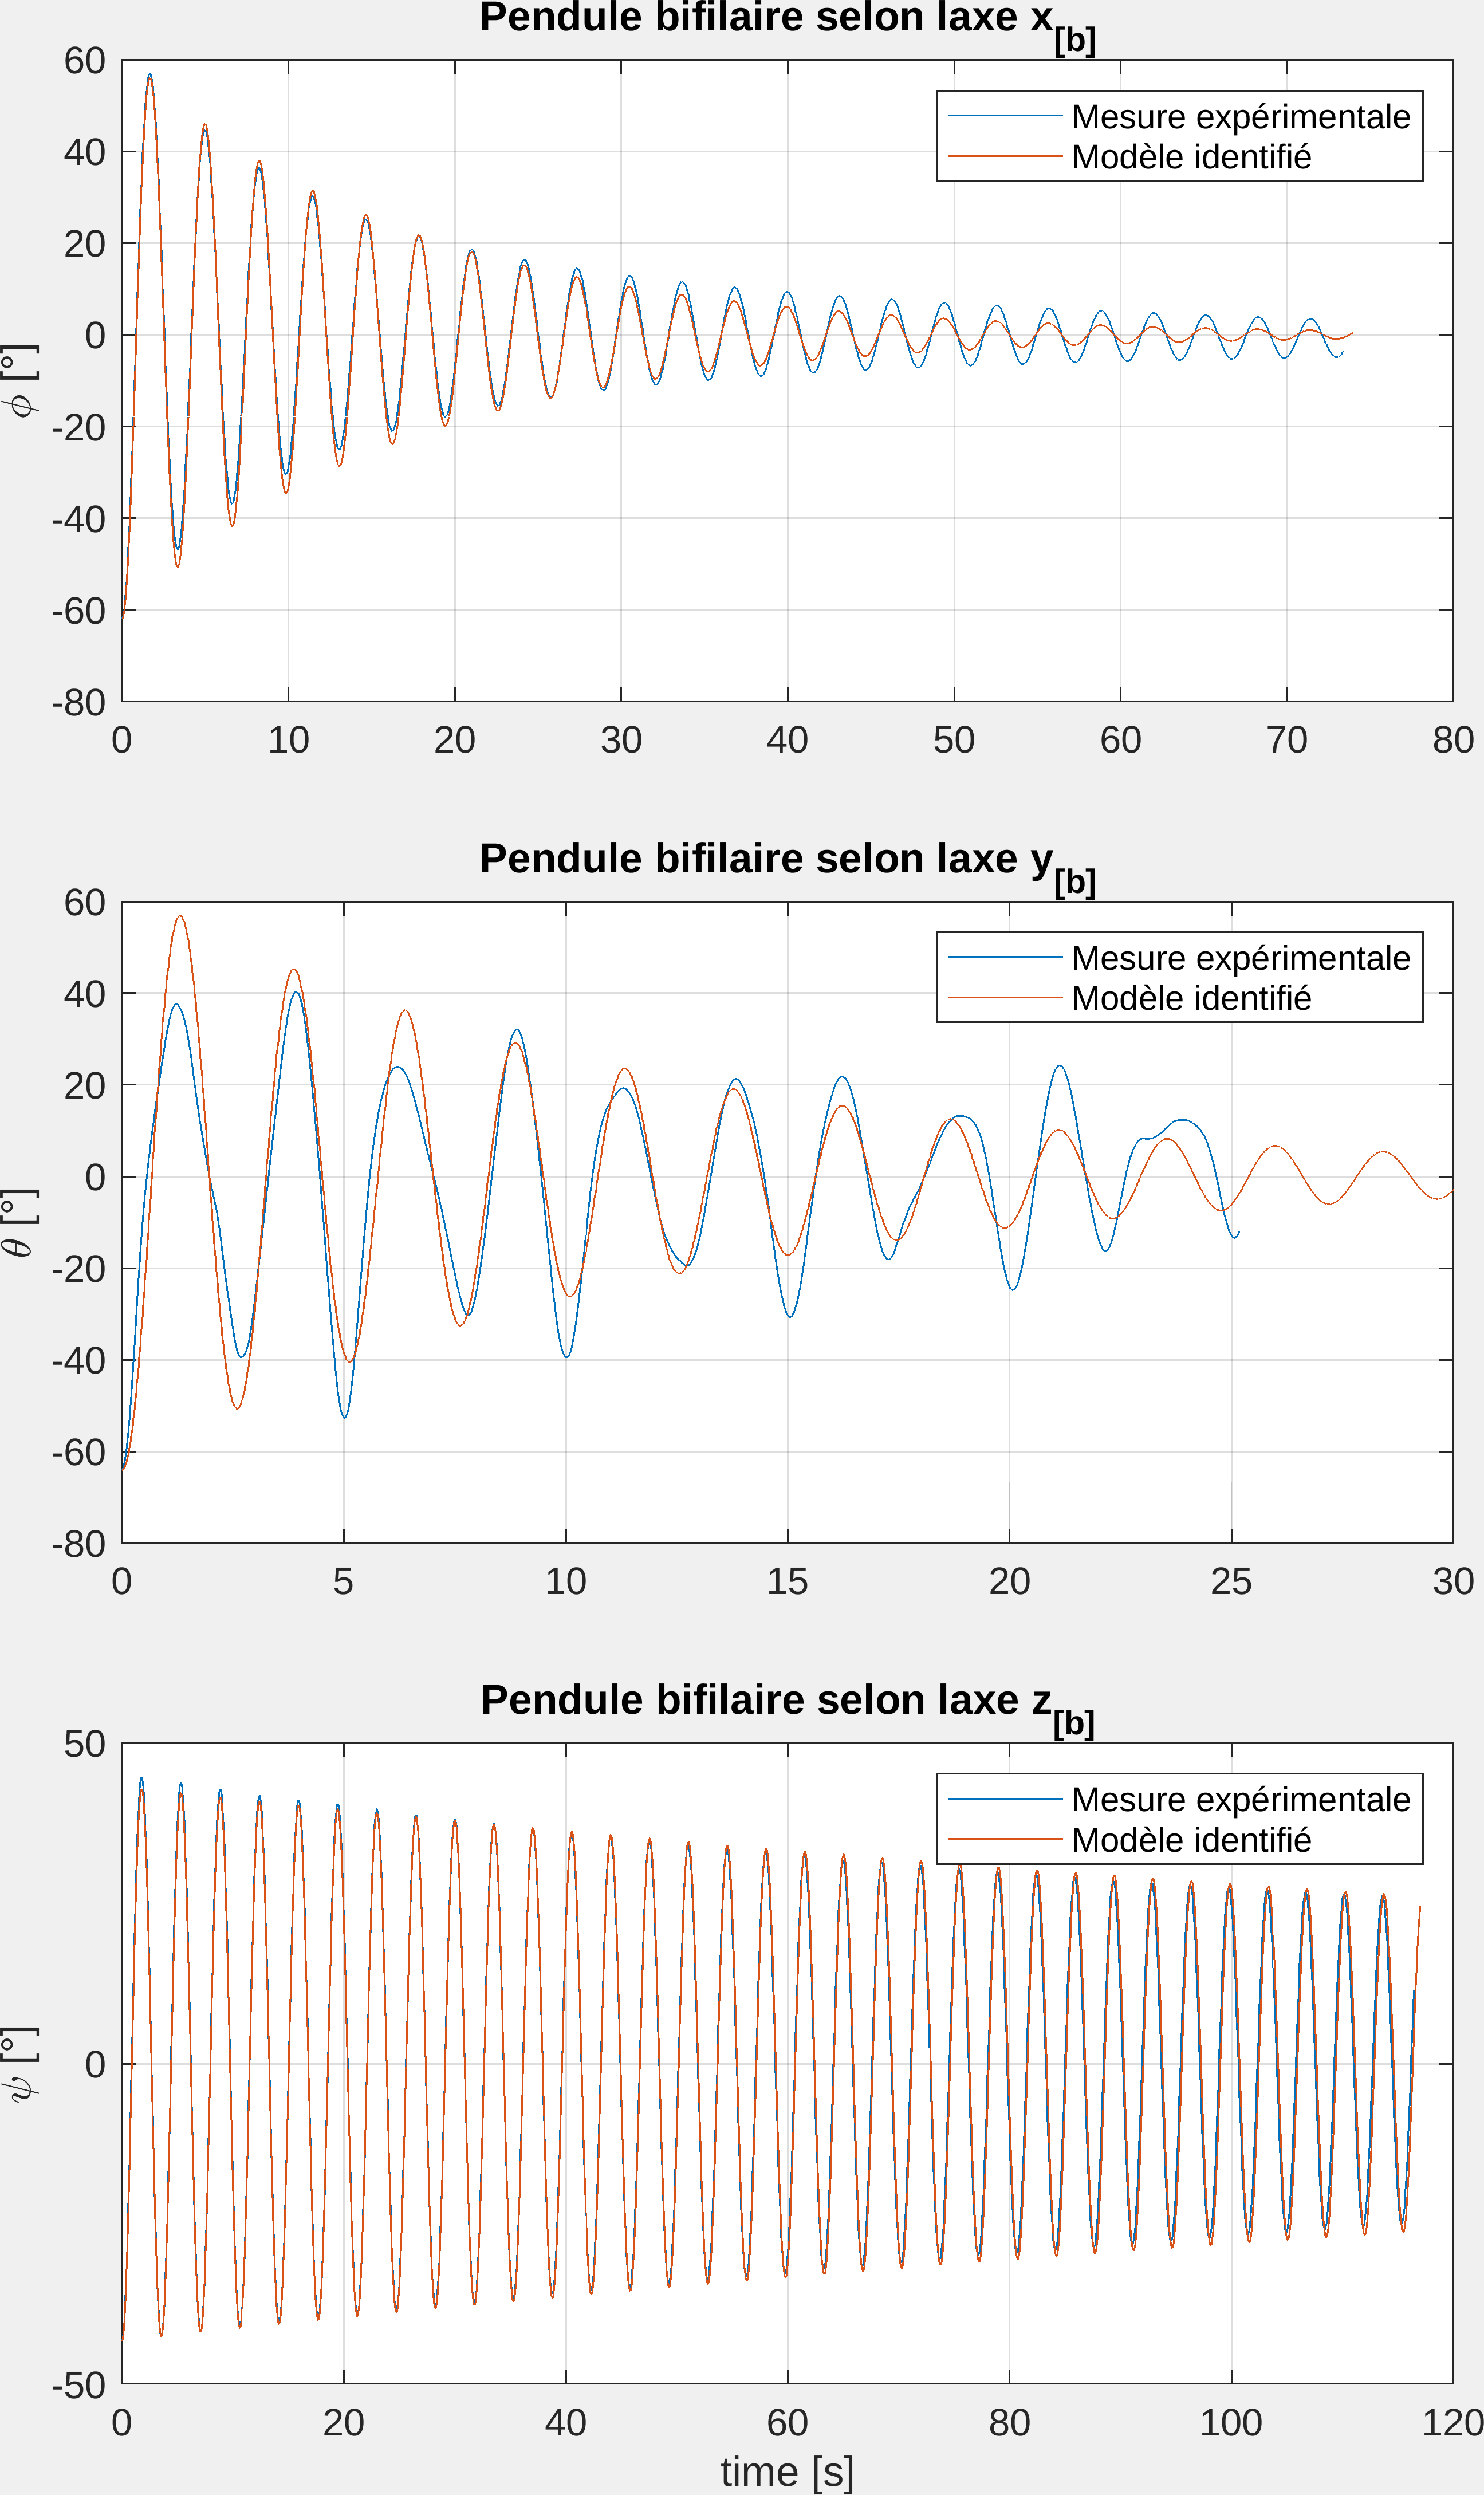
\includegraphics[trim=0cm 0cm 0cm 0cm,clip,width=0.6\columnwidth]{figures/ident_inertia.png}}
    \caption{Bifilar pendulum identication of $\boldsymbol{J}$.}
    \label{fig:BifilarPend_meas}
    \end{figure}
    \todo{ajouter explication sur l'indentification}

\subsection{Modélisation des actionneurs}
    Les actionneurs de DakO ont des dynamqies qui limite leurs actions en terme d'amplitude et de vitesse.

    Pour les moteurs électriques générant la traction par les hélices, il existe deux causes de saturation. Une saturation à haute vitesse liée à  la tension maximale du moteur et une saturation basse vitesse lié à la vitesse minimale de commutation de bobine du moteur pour maintenir la rotation. De plus, ces saturations permettent d'obtenir une modèle réaliste à énergie finie. Elle correspond à la contrainte suivante  $\omega_i \in [2500,~16000]~rpm = [262,~1675]~\SI{}{\radian\per\second}$, $i=1,2$. En termes de dynamique, nous avons représenté la chaîne d'actionnement du moteur (composée de l'ESC, du moteur et de l'hélice) par une fonction de transfert du premier ordre ayant une constante de temps égale à \SI{0,0125}{\second}, ce qui fournit un système d'actionnement assez agressif.

    Les saturations impactant les élevons proviennent des limites physiques des servomoteurs et du débattement limité par la forme de l'UAV, $\delta_i \in [-30~; 30]\text{\textdegree}$, $i=1,2$. La saturation la plus importante ici est peut-être la bande passante de l'actionneur (due à l'actionnement du servomoteur), qui est modélisée par une fonction de transfert du premier ordre avec une constante de temps \SI{0,05}{\second}. 

\section{Équilibres stationnaires}
    \subsection{Équilibre stationnaire sans vent}
    \label{sec:eq_nowind}

    Nous proposons une modification du vecteur de commande, dans le cas d'un équilibre sans vent $\boldsymbol{w}_{\mathrm{eq}} = 0$, basé sur le couplage des actionneurs. 
    \begin{align}
    \boldsymbol{u}_{\text{nowind}} := \begin{bmatrix}\tau_{1}  \!&\! \tau_{2}  \!&\! \delta_{1}\tau_{1} \!&\! \delta_{2}\tau_{2} \end{bmatrix}^\top
    \end{align}
    Nous obtenons un modèle linéaire vis-à-vis de sa commande, dérivé de \eqref{eq:dyna_simp} en imposant  $\boldsymbol{w} = 0$,
    \begin{subequations}\label{eq:withouwind}
    \begin{align}
            \boldsymbol{\dot p} &=  \boldsymbol{v}, \quad &
            m\boldsymbol{\dot v} &= - m\boldsymbol{g} +  \boldsymbol{R}(\boldsymbol{q})\boldsymbol{F}\boldsymbol{u}_{\text{nowind}},\\
            \boldsymbol{\dot q} &= \frac{1}{2}\boldsymbol{q} \otimes \smallmat{0 \\ \boldsymbol{\omega}_{\text{b}}} \quad & \boldsymbol{J} \boldsymbol{\dot \omega}_{\text{b}} &= \! \shortminus \skewsym{\boldsymbol{\omega}_{\text{b}}}\!J\boldsymbol{\omega}_{\text{b}} \! + \! \boldsymbol{M}\boldsymbol{u}_{\text{nowind}},
    \end{align}
    \end{subequations}
    avec les matrices
    \begin{align*}
        \left[ \begin{array}{c|c}\!\boldsymbol{F}\!&\!\boldsymbol{M}\!\end{array} \right] := \left[ \begin{array}{cccc | cccc} a_{\text{f}} & a_{\text{f}} & 0 & 0 & a_{\text{m}} & -a_{\text{m}} & b_{\text{m}} & -b_{\text{m}} \\  0 & 0 & 0 & 0 & 0 & 0 & c_{\text{m}} & c_{\text{m}} \\ 0 & 0 & b_{\text{f}} & b_{\text{f}} & d_{\text{m}} & -d_{\text{m}} & 0 & 0 \end{array} \right]
    \end{align*}
    et les scalaires
        \begin{align*}
            \left[\!\! \begin{array}{c|c} 
            a_{\text{f}} & b_{\text{f}} \\ \hline
            a_{\text{m}} & b_{\text{m}} \\ \hline
            c_{\text{m}} & d_{\text{m}}
            \end{array} \!\!\right] \!=\!
            \left[\begin{array}{c|c}
            1-\frac{S_{\text{wet}}}{4S_{\text{p}}} C_{\text{d}}  & -\frac{S_{\text{wet}}}{4S_{\text{p}}}C_{\ell}\xi_{\text{f}} \\ \hline
            \frac{k_{\text{m}} }{k_{\text{f}}}  &   \! \frac{S_{\text{wet}}}{4S_{\text{p}}}a_{y}C_{\ell}\xi_{\text{f}} \!\\ \hline
            \!\! \frac{S_{\text{wet}}}{4S_{\text{p}}} \Delta_{\text{r}}C_{\ell}\xi_{\text{m}} \!\! & 
            p_{y}+\frac{S_{\text{wet}}}{4S_{\text{p}}} a_{y} C_{\text{d}}
            \end{array}\right].
        \end{align*}


    Tous les couples d'équilibre $(\boldsymbol{u}_{\text{nowind}}, \boldsymbol{x}) = (\boldsymbol{u}_{\text{nowind},\text{eq}}, \boldsymbol{x_{\text{eq}}})$ sont paramétré par une rotation arbitraire autour de l'axe $z_{[\text{i}]}$ définit par $\beta \in \left[-\sqrt{\frac{1}{2}},\sqrt{\frac{1}{2}}\right]$. Le point d'équilibre a pour expression
    \begin{subequations}
        \label{eq:equilibria}
        \begin{align}
            \label{eq:bar_u}
            \boldsymbol{u}_{\text{nowind},\text{eq}} = \frac{mg}{( 1-\frac{S_{\text{wet}}}{4S_{\text{p}}} C_{\text{d}})} [1~1~0~0]^\top\\
            \boldsymbol{q}_{\text{eq}} = [\eta_{\text{eq}} ~\boldsymbol{\epsilon}_{\text{eq}}^\top]^\top = \smallmat{\sqrt{\frac{1}{2}-\beta} & \beta & \frac{2\beta^{2}-1}{2\sqrt{\frac{1}{2}-\beta}} & \beta}^\top.
        \end{align}
    \end{subequations}
    En présence d'un vent nul, le degré de liberté $\beta$ permet d'orienter le drone dans n'importe quelle direction horizontale.

    \subsection{Équilibre stationnaire en présence de vent}
    À partir des modèles \eqref{eq:dyna_orig} et \eqref{eq:dyna_simp}, nous caractérisons un équilibre stationnaire en présence d'un vent constant $\boldsymbol{w}_{\mathrm{eq}} =\smallmat{w_x \\ w_y \\w_z} \in \real^3$ exprimé dans le repère inertiel, tel que $\smallmat{w_x \\ w_y} \neq 0$, c'est-à-dire qu'il existe toujours un vent horizontal non nul.
    Ainsi, pour chaque position de référence $\boldsymbol{p}_{\text{eq}} \in \real^3$, 
    un ensemble de couple état/commande possible est $(\boldsymbol{u}_{\text{eq}}, \boldsymbol{x}_{\text{eq}}) = (\boldsymbol{u}_{\text{eq}}, \boldsymbol{p}_{\text{eq}}, \boldsymbol{v}_{\text{eq}}, \boldsymbol{q}_{\text{eq}}, \boldsymbol{\omega}_{\text{b},\text{eq}})$
    obtenu à l'aide de
    \begin{subequations}
    \label{eq:equilibrium}
    \begin{align}
    \label{eq:ueq}
            &\boldsymbol{u}_{\text{eq}} = \begin{bmatrix} \tau & \tau & \delta & \delta \end{bmatrix}^\top\\
            & \boldsymbol{q}_{\text{eq}} = \boldsymbol{q}_{\mathrm{eq}\psi} \otimes  \boldsymbol{q}_{\mathrm{eq}\theta} \label{eq:qeq}\\
            &\boldsymbol{\omega}_{\text{b},\text{eq}} = 0 , \quad \boldsymbol{v}_{\text{eq}} = 0, 
    \end{align}
    \end{subequations}
    où
    \begin{align}
    \label{eq:qtheta}
        \boldsymbol{q}_{\mathrm{eq}\theta} &:= \begin{bmatrix} \cos(\frac{\theta}{2}) & 0 & \sin(\frac{\theta}{2}) & 0 \end{bmatrix}^\top
    \end{align}
    \todo{traduire et amelioré l'explication}
    we define the quaternion $\boldsymbol{q}_{\mathrm{eq}\psi}$ associated with a horizontal rotation $\psi = \arctan(w_{x}, w_{y})$ of the inertial reference frame towards the (nonzero) horizontal wind direction:

    \begin{align}
    \label{eq:qpsi}
        \boldsymbol{q}_{\mathrm{eq}\psi} &:= \begin{bmatrix} \cos(\frac{\psi}{2}) & 0 & 0 & \sin(\frac{\psi}{2}) \end{bmatrix}^\top.
    \end{align}
    et l'angle d'inclinaison $\theta$, la poussée des hélices $\tau$, et la déflexion des élevons $\delta$ peuvent être obtenu à partir de l'algorithme~\ref{alg:eq}. 

    \begin{algorithm}
    \caption{Obtention des paramètres d'équilibre en \eqref{eq:equilibrium}.}
    \label{alg:eq}
    \hspace*{.1cm} \textbf{Entrée}: Vecteur vent $\boldsymbol{w}_{\text{eq}} =\smallmat{w_x & w_y & w_z}^\top$ \\
    \hspace*{.1cm} \textbf{Sortie}: Paramètres $\psi$, $\theta$, $\tau$, $\delta$ dans \eqref{eq:equilibrium}
    \begin{algorithmic}[1]
        %\Require {\bf Input} values: $\boldsymbol{w} =\smallmat{w_x & w_y & w_z}^\top$ 
        %\Ensure  $\psi$, $\theta$, $\tau$, $\delta$
        \State Détermine l'angle $\psi = \text{atan2}(w_x, w_y)$ de manière à obtenir $\boldsymbol{q}_{\mathrm{eq}\psi}$ dans \eqref{eq:qpsi}  
        \State Détermine la perturbation tournée $\boldsymbol{w}_{\text{r}}$ avec la composante $y$ nulle, en utilisant $\boldsymbol{R}_{\psi}:= \smallmat{ \cos \psi & \sin \psi & 0 \\ -\sin \psi & \cos \psi & 0 \\ 0 & 0 & 1 }$, selon
        \begin{align}
        \label{eq:wh}
        \boldsymbol{w}_{\mathrm{r,eq}} := \smallmat{w_{\text{r}x} \\ 0 \\w_{\text{r}z}} :=  \boldsymbol{R}^\top(\boldsymbol{q}_{\mathrm{eq}\psi}) \boldsymbol{w}_{\mathrm{eq}} = \boldsymbol{R}^\top_{\psi} \boldsymbol{w}_{\mathrm{eq}}
        \end{align}

        \State Détermine l'angle d'inclinaison $\theta$ de manière à obtenir $\boldsymbol{q}_{\text{eq}\theta}$ dans \eqref{eq:qeq}:  
        \begin{align}
        \label{eq:theta_alg}
            \theta = -\tan^{-1}\left(\frac{w_{\text{r}z}}{w_{\text{r}x}} + \frac{2mg}{\rho S \lVert \boldsymbol{w}_{\mathrm{eq}} \rVert C_{\ell}  (1-\frac{\xi_{\text{f}}}{\xi_{\text{m}}}) w_{\text{r}x} } \right)
        \end{align}
    \State Pour des raisons de commodité, nous définissons les scalaires 
        $$ 
        \left[\begin{array}{c|c} 
        \!\!a\!\!&\!\!b\!\! \\ \hline \!\!c\!\!&\!\! d\!\!\end{array}  \right] \!:=\! 
        \left[\begin{array}{c|c}
        2 S_{\text{wet}} C_{\ell} mg \sin{\theta} \xi_{\text{f}} &
        \! 2 S_{\text{wet}} C_{\text{d}} C_{\ell} \rho  \lVert \boldsymbol{w}_{\mathrm{eq}} \rVert  w_{x}^{\text{b}}\!\! \\ \hline
        \!\!-4 S S_{\text{p}} C_{\ell} \rho  \lVert \boldsymbol{w}_{\mathrm{eq}} \rVert  w_{x}^{\text{b}} \xi_{\text{f}}\!\! & \frac{b \xi_{\text{f}}}{2}
        \end{array}\right]
        $$ 
        et grâce à ces scalaires $(a,b,c,d)$, déterminons la traction des hélices $\tau$ dans \eqref{eq:ueq} comme
        \begin{align}
            \nonumber
            \tau &= \frac{S_{\text{p}}}{2 S_{\text{wet}} C_{\ell} \xi_{\text{f}} (4S_{\text{p}} -  S_{\text{wet}} C_{\text{d}} )} \Bigg( a+b+c+d + \Bigg[ (a+b+c \shortminus d)^2 \shortminus 4 (d^2+ac \shortminus bd)  \\ 
            & \quad
            \shortminus \frac{4 {w_{z}^{\text{b}}}^2 d}{ {w_{x}^{\text{b}}}^2 } (d+c) + \frac{4 w_{z}^{\text{b}}ad\cos{\theta}}{w_{x}^{\text{b}} C_{\ell} \sin{\theta} } \left(C_{\text{d}} - \frac{4 S_{\text{p}}}{S_{\text{wet}}}\right) \Bigg] ^{\frac{1}{2}} \Bigg),\label{eq:tau_alg}
        \end{align}
        où
        $$
        \bigmat{w_{x}^{\text{b}} \\ w_{z}^{\text{b}}} = \bigmat{   w_{\text{r}x} \cos{\theta} - w_{\text{r}z} \sin{\theta}\\
                    w_{\text{r}x} \sin{\theta} +  w_{\text{r}z} \cos{\theta} }.
        $$
        
        \State Déterminons la déflexion des élevons $\delta$ comme
        \begin{align}
        \label{eq:delta_alg}
            \delta = \frac{2mg\sin{\theta}}{\rho S \lVert \boldsymbol{w}_{\mathrm{eq}} \rVert C_{\text{d}}\xi_{\text{f}} w_{z}^{\text{b}}} + \frac{w_{x}^{\text{b}}}{\xi_{\text{f}}w_{z}^{\text{b}}} -  \frac{(4-\frac{S_{\text{wet}}}{S_{\text{p}}} C_{\text{d}})}{\rho S \lVert \boldsymbol{w}_{\mathrm{eq}} \rVert C_{\text{d}}\xi_{\text{f}} w_{z}^{\text{b}}} \tau.
        \end{align}

    \end{algorithmic}
    \hspace*{.1cm} \textbf{Retourne}:  $\psi$, $\theta$, $\tau$, $\delta$
    \end{algorithm}


    \begin{theorem}\label{thm:eqs}
    Pour tout vent constant, $\boldsymbol{w} =\smallmat{w_x & w_y & w_z}^\top \in \real^3$ ayant une composante horizontale non nulle $\smallmat{w_x \\ w_y}$,
    les equations \eqref{eq:qpsi}--\eqref{eq:qtheta} avec $\theta$, $\tau$ et $\delta$ sélectionné selon l'Algorithme~\ref{alg:eq} caractérisent un couple d'équilibre $(\boldsymbol{u}_{\text{eq}}, \boldsymbol{x}_{\text{eq}})$ pour la dynamique non linéaire \eqref{eq:dyna_orig} et \eqref{eq:dyna_simp}.
    
    \end{theorem}
    
    \begin{proof}
        Dans un premier temps, notons qu'avec l'expression de $\boldsymbol{R}$ \eqref{eq:matrix_rot} et l'expression de  $\psi$ dans l'étape 1 de l'Algorithme~\ref{alg:eq}, on peut définir la perturbation à l'équilibre tournée $\boldsymbol{w}_{\mathrm{r,eq}} := \boldsymbol{R}^\top_{\psi} \boldsymbol{w}_{\mathrm{eq}} :=    \boldsymbol{R}^\top(\boldsymbol{q}_{\mathrm{eq}\psi})\boldsymbol{w}_{\mathrm{eq}}$ (voir \eqref{eq:wh} dans l'Algorithme~\ref{alg:eq}),
        qui correpond à la rotation necessaire pour aligner l'axe  $x_{[\text{b}]}$ du repère corps avec la direction du vent. Une fois que le drone est face au vent, il subit un vent avec une composante latérale $y$ nulle et il peut ajuster son angle d'inclinaison $\theta$ afin de générer la poussée et la portance nécessaires pour compenser les effets du vent dans les directions longitudinale et verticale (l'effet latéral est nul en raison de l'orientation spécifique de l'appareil $\psi$). Avec cette rotation $\psi$, il est possible d'exprimer le vent dans le repere corps comme étant
            \begin{align}
            \label{eq:wb}
                \boldsymbol{w}^{\text{b}}_{\mathrm{eq}} &:= 
                \begin{bmatrix}
                    w_{x}^{\text{b}} \\ 0 \\ w_{z}^{\text{b}}
                \end{bmatrix} \!=\! 
                \boldsymbol{R}^\top(\boldsymbol{q}_{\text{eq}\theta}) \boldsymbol{w}_{\mathrm{r,eq}}  \\
                &=\!\! \begin{bmatrix}
                    \cos{\theta} & 0 & -\sin{\theta}\\
                        0 & 1 & 0\\
                    \sin{\theta} & 0 & \cos{\theta}
                \end{bmatrix}^\top \!\! \begin{bmatrix}
                    w_{\text{r}x}\\
                    0\\
                    w_{\text{r}z}
                \end{bmatrix}
                \!\!=\!\!\begin{bmatrix}
                    w_{\text{r}x} \cos{\theta} - w_{\text{r}z} \sin{\theta}\\
                    0\\
                    w_{\text{r}x} \sin{\theta} +  w_{\text{r}z} \cos{\theta}
                \end{bmatrix}
            \nonumber
            \end{align}
        Nous insistons sur le fait que $w_{x}^{\text{b}}$ est toujours négatif et différent de zéro, car le drone est orienté dans la direction du vent grâce à la rotation engendré par $ \boldsymbol{q}_{\mathrm{eq}\psi}$, et suite à l'hypothèse $\smallmat{w_x \\ w_y} \neq 0$.
    
        L'équation \eqref{eq:dyna1} montre qu'il est nécessaire d'avoir $\boldsymbol{v}_{\text{eq}} = 0$ pour maintenir l'équilibre stationnaire. En multipliant \eqref{eq:dyna2} par $\boldsymbol{R}(\boldsymbol{q}_{\text{eq}})$ donné dans  \eqref{eq:wb}, nous l'exprimons dans le repère corps.
        Comme nous appliquons la même commande $\tau_{1} = \tau_{2} = \tau $ aux deux moteurs et la même commande au deux élevons $\delta_{1} = \delta_{2} = \delta$, nous obtenons pour les deux modèles \eqref{eq:dyna_orig} et \eqref{eq:dyna_simp}, l'équilibre des forces selon l'axe $x_{[\text{b}]}$ donné par
        \begin{align}
            & (2-\frac{S_{\text{wet}}}{2S_{\text{p}}} C_{\text{d}})\tau - \frac{1}{2}\rho S \lVert \boldsymbol{w}_{\mathrm{eq}} \rVert C_{\text{d}} \left(w_{x}^{\text{b}} - \xi_{\text{f}} \delta w_{z}^{\text{b}} \right) - mg \sin(\theta) = 0 \label{eq:forcex}
        \end{align}
        et l'équilibre des forces selon l'axe $z_{[\text{b}]}$ donné par
        \begin{align}\label{eq:forcez}
            - \frac{S_{\text{wet}}}{2S_{\text{p}}}\xi_{\text{f}} C_{\ell} \tau \delta - \frac{1}{2}\rho S \lVert \boldsymbol{w}_{\mathrm{eq}} \rVert C_{\ell} \left(w_{z}^{\text{b}} + \xi_{\text{f}} \delta w_{x}^{\text{b}} \right) + mg \cos(\theta) = 0
        \end{align}
        De manière similaire, à partir de \eqref{eq:dyna_orig_b} et \eqref{eq:dyna4}, l'équilibre des moments autour de l'axe $y_{[\text{b}]}$ permet d'obtenir
        \begin{align}\label{eq:momenty}
            \frac{S_{\text{wet}}}{2S_{\text{p}}}  \Delta_{\text{r}} \xi_{\text{m}} C_{\ell} \tau \delta + \frac{1}{2}\rho S \Delta_{\text{r}} \lVert \boldsymbol{w}_{\mathrm{eq}} \rVert C_{\ell} \left(w_{z}^{\text{b}} + \xi_{\text{m}} \delta w_{x}^{\text{b}} \right) = 0.
        \end{align}
        
        Pour calculer la solution du triplet ($\theta$,$\tau$,$\delta$) des trois équations d'équilibre \eqref{eq:forcex}--\eqref{eq:momenty}, ajoutons \eqref{eq:forcez} multiplié par $\Delta_{\text{r}} \xi_{\text{m}}$, à \eqref{eq:momenty} multiplié par $\xi_{\text{f}}$, de manière à annuler le premier terme et à obtenir
        \begin{multline*}
            \Delta_{\text{r}} \xi_{\text{m}} \left( - \frac{1}{2}\rho S \lVert \boldsymbol{w}_{\mathrm{eq}} \rVert C_{\ell} (w_{z}^{\text{b}} + \xi_{\text{f}} \delta w_{x}^{\text{b}}) + mg \cos(\theta) \right) \\+ \xi_{\text{f}} \left(\frac{1}{2}\rho S  \Delta_{\text{r}} \lVert \boldsymbol{w}_{\mathrm{eq}} \rVert C_{\ell} (w_{z}^{\text{b}} + \xi_{\text{m}} \delta w_{x}^{\text{b}})  \right) = 0,
        \end{multline*}
        qui est équivalent à
        \begin{align*}
            \frac{1}{2}\rho S  \Delta_{\text{r}} \lVert \boldsymbol{w}_{\mathrm{eq}} \rVert C_{\ell}  (\xi_{\text{f}} - \xi_{\text{m}}) w_{z}^{\text{b}} +   \Delta_{\text{r}} \xi_{\text{m}} mg \cos(\theta)  = 0,
        \end{align*}
        où ($w_{x}^{\text{b}}$,$w_{z}^{\text{b}}$) sont les première et troisième composantes de $\boldsymbol{w}^{\text{b}}$ dans \eqref{eq:wb}. Ensuite, en utilisant \eqref{eq:wb} et en réarrangeant, nous obtenons
        \begin{multline*}
                -\frac{1}{2}\rho S  \Delta_{\text{r}} \lVert \boldsymbol{w}_{\mathrm{eq}} \rVert C_{\ell}  (\xi_{\text{f}} - \xi_{\text{m}}) w_{\text{r}x} \sin{\theta}  +\bigg( -\frac{1}{2}\rho S  \Delta_{\text{r}} \\ \lVert \boldsymbol{w}_{\mathrm{eq}} \rVert C_{\ell}  (\xi_{\text{f}} - \xi_{\text{m}})w_{\text{r}z} +   \Delta_{\text{r}} \xi_{\text{m}} mg \bigg) \cos{\theta} = 0,
        \end{multline*}
        qui est satisfaite par
            \begin{align} \label{eq:theta}
                \theta &=  -\tan^{-1}\left(\frac{\rho S \lVert \boldsymbol{w}_{\mathrm{eq}} \rVert C_{\ell}  (\xi_{\text{f}} - \xi_{\text{m}})w_{\text{r}z} - 2 \xi_{\text{m}} mg }{\rho S\lVert \boldsymbol{w}_{\mathrm{eq}} \rVert C_{\ell}  (\xi_{\text{f}} - \xi_{\text{m}}) w_{\text{r}x}}\right).
            \end{align}
            Cette dernière expression coïncide avec la sélection \eqref{eq:theta_alg} dans l'Algorithme~\ref{alg:eq} après quelques manipulations.
        À partir de \eqref{eq:theta_alg}, nous pouvons calculer les commandes à l'équilibre en substituant \eqref{eq:forcex} dans \eqref{eq:forcez}. Après quelques simplifications, la force nécessaire de traction des hélices  $\tau$ pour maintenir la position d'équilibre corresponds à l'expression  \eqref{eq:tau_alg}. Finalement, avec la valeur de $\tau$ dans \eqref{eq:tau_alg}, nous pouvons obtenir la déflexion des élevons nécessaire $\delta$ à partir de l'équation \eqref{eq:forcez}, ce qui nous donne la valeur obtenue dans \eqref{eq:delta_alg}.
    \end{proof}
    Il est intéressant de noter que pour chaque couple de vent($w_{\text{r}z}$, $w_{\text{r}x}$) correspond une orientation d'équilibre \eqref{eq:qeq}, \eqref{eq:theta_alg} est indépendante de l'entrée $\boldsymbol{u}_{\text{eq}}$. En outre, il convient de souligner que pour toutes les valeurs de vent raisonnables, l'équation \eqref{eq:tau_alg} correspond à la racine positive d'un polynôme du second ordre, l'autre racine étant toujours négative, ce qui conduit à une condition de poussée négative physiquement impossible.


    À partir de l'expression analytique \eqref{eq:equilibrium} de l'équilibre du drone pour différentes conditions de vent $\boldsymbol{w}$, nous reportons, sur la Fig. \ref{fig:saturation}, les valeurs correspondantes de $\theta$, $\delta$, $\tau$ pour des valeurs de vitesse de vent horizontale allant de 0 à \SI{-20}{\meter\per\second} et pour des valeurs de vitesse de vent verticale allant de \SI{-6}{} à \SI{6}{\meter\per\second}. L'angle d'incidence $\theta$ diminue de \SI{90}{\degree} à \SI{-4.65}{\degree}. $\theta = \SI{90}{\degree}$ correspond à un vol stationnaire sans vent. La traction $\tau$ atteint son minimum à $w_{rx} = \SI{-12.8}{\meter\per\second}$, ce qui correspond à une condition de vol qui minimise la consommation d'énergie, car les moteurs sont la principale source de consommation électrique.
        
    \todo{traduction caption}
    \begin{figure}[ht!]
        \centering
        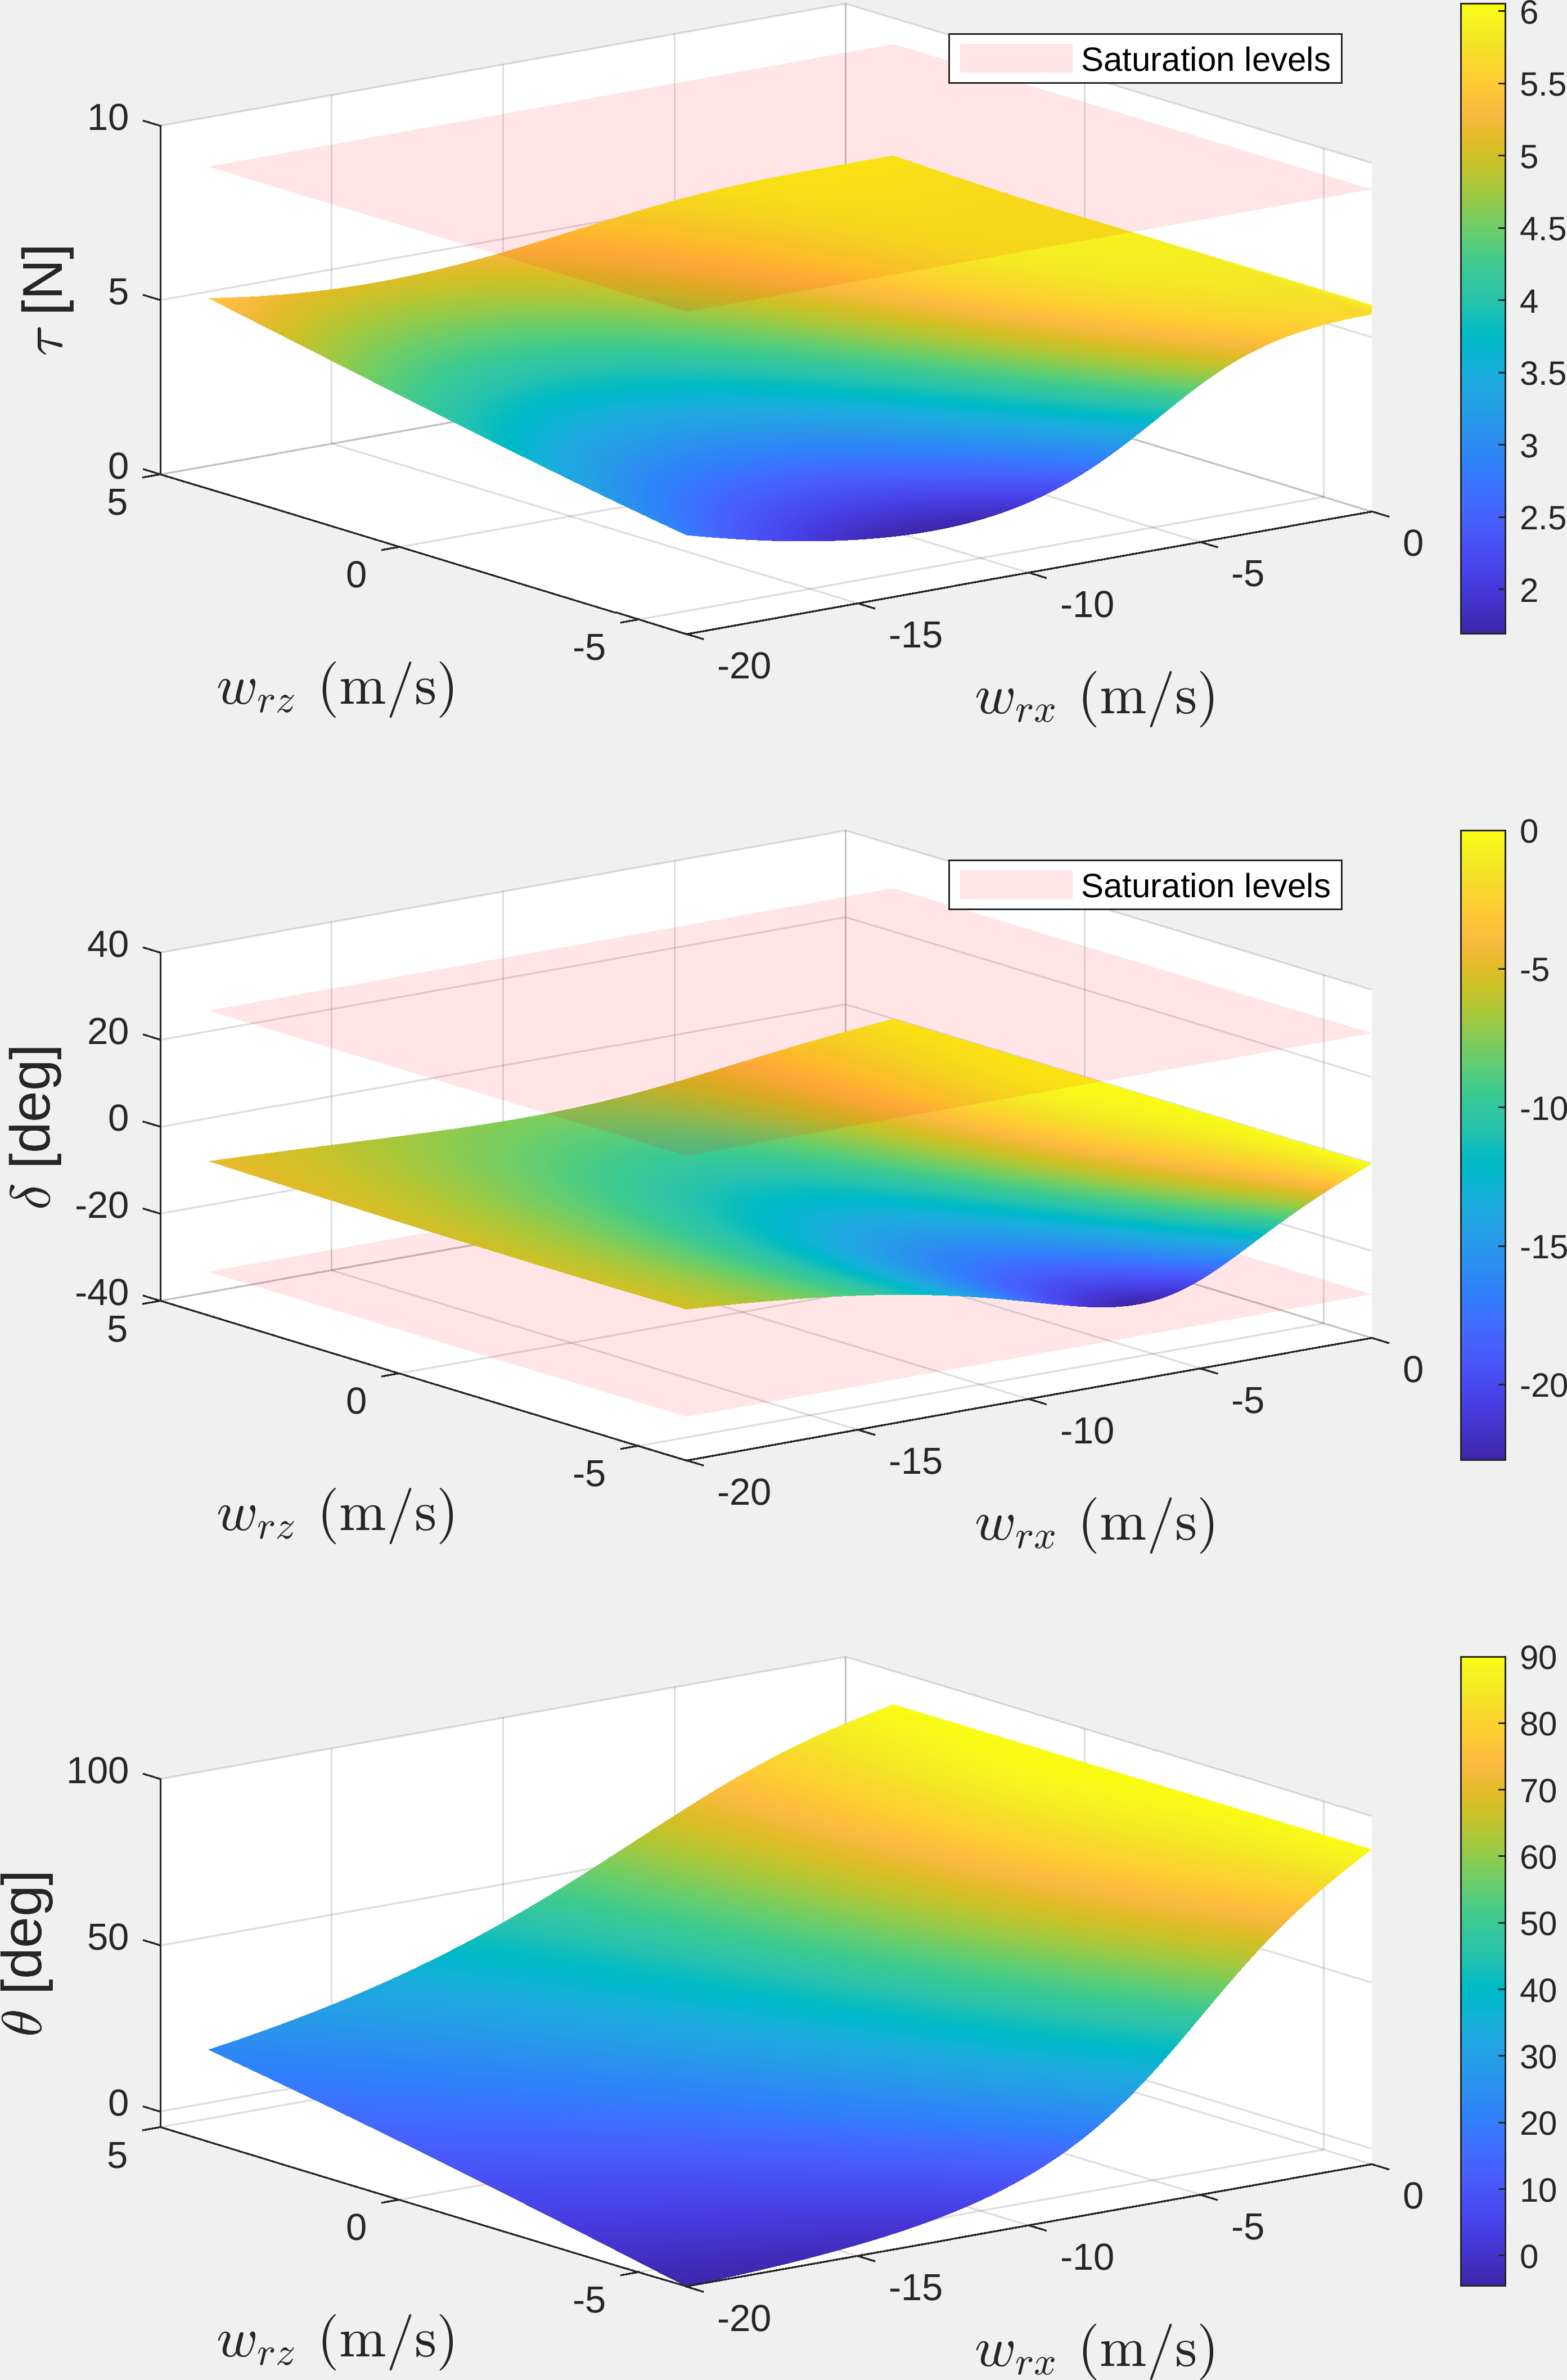
\includegraphics[trim=0cm 0cm 0cm 0cm,clip,width=0.5\columnwidth]{figures/equilibrium_wx_wz.png}
        \caption{Parameters ($\theta$, $\delta$, $\tau$) of the equilibrium point (surface) established in Theorem~\ref{thm:eqs} and Algorithm \ref{alg:eq} for constant horizontal and vertical wind ($w_{\text{r}x}$,$w_{\text{r}z}$), and actuators saturation levels (red).}
        \label{fig:saturation}
    \end{figure}
    Il est possible de faire une coupe des surfaces présentée dans \eqref{fig:saturation} pour une vitesse verticale nulle $\boldsymbol{w}_{\text{rx}} = 0$, ce qui nous donne le résultat de la Figure \ref{fig:saturation_wz0}
    \begin{figure}[ht!]
        \centering
        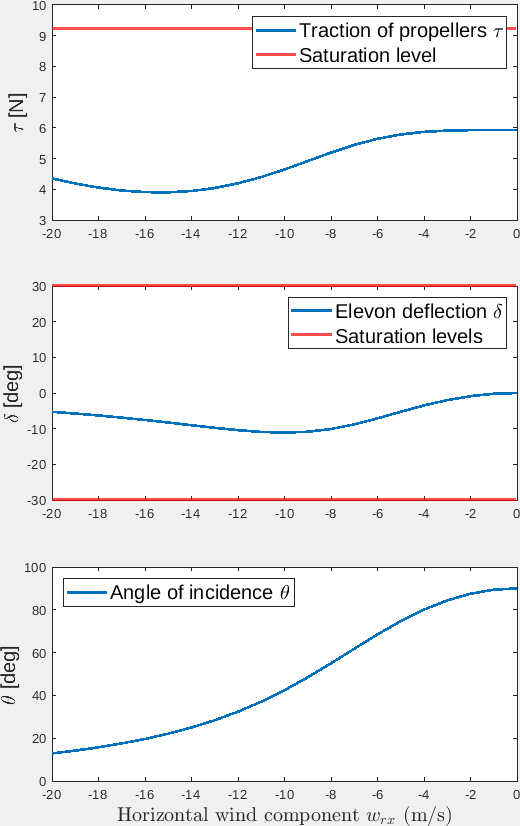
\includegraphics[trim=0cm 0cm 0cm 0cm,clip,width=0.5\columnwidth]{figures/equilibrium.png}
        \caption{Parameters ($\theta$, $\delta$, $\tau$) of the equilibrium point (blue) established in Theorem~\ref{thm:eqs} and Algorithm \ref{alg:eq} for a constant horizontal wind $w_{\text{r}x}$, and actuators saturation levels (red).}
        \label{fig:saturation_wz0}
    \end{figure}

\section{Dynamiques linéarisés}
\subsection{Dynamique linéarisé sans vent}
Considérons le cas sans vent discuté dans la section \ref{sec:eq_nowind} pour lequel nous utilisons le vecteur de commande $\boldsymbol{u}_{\text{nowind}}$  et le vecteur de commande à l'équilibre $\boldsymbol{u}_{\text{nowind},\text{eq}}$ défini dans l'équation \eqref{eq:bar_u} et rapellons la transformation du vecteur de comamande suivante $ \boldsymbol{u}_{\text{nowind}} := \begin{bmatrix}\tau_{1}  \!&\! \tau_{2}  \!&\! \delta_{1}\tau_{1} \!&\! \delta_{2}\tau_{2} \end{bmatrix}^\top$, la dynamqiue linearisé dans le cas sans vent est 
\begin{align}
    \label{eq:linearized}
     \boldsymbol{\dot{\tilde{x}}} = \boldsymbol{A}_{0} \tilde{\boldsymbol{x}} + \boldsymbol{G}_{0} (\boldsymbol{u}_{\text{nowind}}-\boldsymbol{u}_{\text{nowind},\text{eq}}),
\end{align}
où l'expression de $\boldsymbol{A}_{0}$ est
\begin{align}
    \label{matrice_A}
        \boldsymbol{A}_{0} = \boldsymbol{A}_{w} \Big|_{\boldsymbol{w}=0} =\begin{bmatrix}
        \mathbb{0}_{3} & \mathbb{I}_{3} & \mathbb{0}_{3} & \mathbb{0}_{3} \\
        \mathbb{0}_{3} & \mathbb{0}_{3} &  \boldsymbol{A}_{v\epsilon} & \mathbb{0}_{3} \\
        \mathbb{0}_{3} & \mathbb{0}_{3} & \mathbb{0}_{3} & \boldsymbol{A}_{\epsilon\omega} \\
        \mathbb{0}_{3} & \mathbb{0}_{3} & \mathbb{0}_{3} & \mathbb{0}_{3}
        \end{bmatrix},
\end{align}
avec les matrices suivante
\begin{align*}
    \boldsymbol{A}_{\epsilon\omega} = \frac{\sqrt{2}}{4}\begin{bmatrix} 
        1 & 0 & -1 \\ 
        0 & 1 & 0  \\
       1 & 0 & 1
    \end{bmatrix} \text{ and } \boldsymbol{A}_{ v\epsilon} = \sqrt{2}\begin{bmatrix} 
        0 & -2g & 0\\
        g & 0 & g  \\ 
         0 & -2g & 0 \end{bmatrix},
\end{align*}
while the expression of $\boldsymbol{G}_{0}$ is 
\begin{align*}
    \boldsymbol{G}_{0}  := \begin{bmatrix}
    \mathbb{0}_{3\times 1} & \mathbb{0}_{3\times 1} & \mathbb{0}_{3\times 1} & \mathbb{0}_{3\times 1}\\
    0 & 0 & a_{\text{g}} & a_{\text{g}}\\
    0 & 0 & 0 & 0\\
    b_{\text{g}} & b_{\text{g}}  & 0 & 0\\
    \mathbb{0}_{3\times 1} & \mathbb{0}_{3\times 1} & \mathbb{0}_{3\times 1} & \mathbb{0}_{3\times 1}\\
    c_{\text{g}} & -c_{\text{g}} & d_{\text{g}} & -d_{\text{g}}\\
    0 & 0 & e_{\text{g}} & e_{\text{g}}\\
    f_{\text{g}} & -f_{\text{g}} & 0 & 0\\
    \end{bmatrix} , 
\end{align*}
with
\begin{align*}
    \left[\!\! \begin{array}{c|c} 
    a_{\text{g}} & b_{\text{g}} \\ \hline
    c_{\text{g}} & d_{\text{g}} \\ \hline
    e_{\text{g}} & f_{\text{g}}
    \end{array} \!\!\right] \!=\!
    \left[\begin{array}{c|c}
   \shortminus \frac{S_{\text{wet}}}{4mS_{\text{p}}}C_{\ell}\xi_{\text{f}}  & \frac{1}{m}( 1-\frac{S_{\text{wet}}}{2S_{\text{p}}} C_{\text{d}}) \\ \hline
    \frac{k_{\text{m}} }{J_{x}k_{\text{f}}}  &   \! \frac{ S_{\text{wet}} a_{y} }{4 J_{x} S_{\text{p}} } C_{\ell}\xi_{\text{f}} \!\\ \hline
    \!\! \frac{S_{\text{wet}}\Delta_{\text{r}}}{4J_{y}S_{\text{p}}} C_{\ell}\xi_{\text{m}} \!\! & 
    \frac{1}{J_{z}}(p_{y}\!+\!\frac{S_{\text{wet}}}{4S_{\text{p}}} a_{y} C_{\text{d}})\!\!
    \end{array}\right].
\end{align*}
We emphasize that these equations coincide with the expressions given in our preliminary work \cite[eqn. (22)]{sansou:ECC}.



\subsection{Dynamique linéarisé en présence de vent}

For each one of the equilibria characterized in Theorem~\ref{thm:eqs}, we derive here some linearized equations of motion with respect to the simplified nonlinear low-speed model \eqref{eq:dyna_simp}. A direct approach would lead to linearized equations that depend on the $\psi$ angle characterized in step 1 of Algorithm~\ref{alg:eq}.
Instead, we define here the incremental coordinates in a suitably rotated inertial reference frame, so that the linearized dynamics is independent of the $\psi$ angle .
More specifically, for each equilibrium wind condition $\boldsymbol{w}_{\text{eq}}$ and the ensuing equilibrium
$(\boldsymbol{u}_{\text{eq}}, \boldsymbol{p}_{\text{eq}},
\boldsymbol{q}_{\text{eq}})$ characterized in \eqref{eq:qpsi}--\eqref{eq:qtheta}, 
denoting the scalar and vector components of the quaternion in \eqref{eq:qeq} as
$\boldsymbol{q}_{\text{eq}} = (\eta_{\text{eq}}, \boldsymbol{\epsilon}_{\text{eq}})$, and
based on the rotation matrix
$\boldsymbol{R}_{\psi} :=    \boldsymbol{R}(\boldsymbol{q}_{\mathrm{eq}\psi})$ introduced at the beginning of the proof of Theorem~\ref{thm:eqs}, we study here the approximate linear dynamics of the rotated incremental input-state vector:  
\begin{align}
\label{eq:xtilde}
     \nonumber &\tilde{\boldsymbol{x}} := (\tilde{\boldsymbol{p}},
     \tilde{\boldsymbol{v}},
     \tilde{\boldsymbol{\epsilon}},
     \tilde{\boldsymbol{\omega}}_{\text{b}}) = \left(\boldsymbol{R}^\top_{\psi} (\boldsymbol{p} \! \shortminus \! \boldsymbol{p}_{\text{eq}}), \boldsymbol{R}^\top_{\psi} \boldsymbol{v}, \boldsymbol{R}^\top_{\psi} (\boldsymbol{\epsilon} \! \shortminus \! \boldsymbol{\epsilon}_{\text{eq}}), \boldsymbol{\omega}_{\text{b}} \right), \\ &\tilde{\boldsymbol{u}} := \boldsymbol{u}-\boldsymbol{u_{\text{eq}}}, \quad \tilde{\boldsymbol{w}} := \boldsymbol{R}^\top_{\psi} (\boldsymbol{w}-\boldsymbol{w}_{\mathrm{eq}}).
\end{align}
Note that the rotation in \eqref{eq:xtilde} enjoys the useful property that $\boldsymbol{R}^\top_{\psi} \boldsymbol{\epsilon}_{\text{eq}} = \smallmat{0 & \sin(\frac{\theta}{2}) & 0}^\top$, a fact that greatly simplifies the linearized motion.


% the constants $\boldsymbol{p}_{\text{eq}} \in \real^3$, $\boldsymbol{u}_{\text{eq}} \in \real^4$ and $\boldsymbol{\epsilon}_{\text{eq}} \in \real^3$ come from any of the equilibrium pairs characterized in Theorem~\ref{thm:eqs} (see equation \eqref{eq:equilibrium})) and $\boldsymbol{u}$ in equation \eqref{eq:vector_u}).


Exploiting the fact that the translational and rotational speeds ($\boldsymbol{v}_{\text{eq}}$, $\boldsymbol{\omega}_{\text{b,eq}})$ must be zero at the equilibrium (see \eqref{eq:equilibrium}), we prove below that the approximate linearized dynamics for 
the state in \eqref{eq:xtilde} is given by
% about $\boldsymbol{x}_{\text{eq}}$ is given by
%
\begin{align}
\label{eq:lpv_linearisation}
 \boldsymbol{\dot{\tilde{x}}} &= \boldsymbol{A}_{w} \tilde{\boldsymbol{x}} + \boldsymbol{G}_{w} \tilde{\boldsymbol{u}} + \boldsymbol{E}_{w}  \tilde{\boldsymbol{w}} \\
 &= \smallmat{
     \mathbb{0}_{3} & \mathbb{I}_{3} & \mathbb{0}_{3} &\mathbb{0}_{3} \\
    \mathbb{0}_{3} & \boldsymbol{A}_{vv}  & \boldsymbol{A}_{v\epsilon}  & \mathbb{0}_{3}\\
    \mathbb{0}_{3} & \mathbb{0}_{3} & \mathbb{0}_{3} & \boldsymbol{A}_{\epsilon \omega} \\    
    \mathbb{0}_{3} & \mathbb{0}_{3} &  \boldsymbol{A}_{\omega \epsilon} & \mathbb{0}_{3}
    } \tilde{\boldsymbol{x}} \!+\!
    \smallmat{ \mathbb{0}_{3 \times 4} \\
     \boldsymbol{G}_{v}\\
     \mathbb{0}_{3 \times 4}\\
     \boldsymbol{G}_{\omega}
    } \tilde{\boldsymbol{u}}
    \!+\! \smallmat{
     \mathbb{0}_{3 \times 3} \\
     \boldsymbol{E}_{v} \\
     \mathbb{0}_{3 \times 3} \\
     \boldsymbol{E}_{\omega} 
     } \!\tilde{\boldsymbol{w}},
     \nonumber
\end{align}
%
with matrices $\boldsymbol{A}_{vv} $, $\boldsymbol{A}_{v\epsilon}$, $\boldsymbol{A}_{\epsilon \omega_{\text{b}}}$, $\boldsymbol{A}_{\omega \epsilon}$, $ \boldsymbol{G}_{v}$, $\boldsymbol{G}_{\omega}$ $\boldsymbol{E}_{v}$, $\boldsymbol{E}_{\omega}$ constructed by following Algorithm~\ref{alg:linea}.

\begin{theorem} \label{th:lin}
For any constant wind, $\boldsymbol{w} =\smallmat{w_x & w_y & w_z}^\top \in \real^3$ having a nonzero horizontal component $\smallmat{w_x \\ w_y}$, and the ensuing equilibrium pair $(\boldsymbol{u}_{\text{eq}}, \boldsymbol{x}_{\text{eq}})$ of dynamics \eqref{eq:dyna_simp}, as
characterized in \eqref{eq:qpsi}-\eqref{eq:qtheta}, the linearized dynamics of 
the incremental input-state vector \eqref{eq:xtilde}
% \eqref{eq:dyna_simp_rot}) about $\boldsymbol{x_{\text{eq}}}$
is given by \eqref{eq:lpv_linearisation} with the matrices constructed as in Algorithm~\ref{alg:linea}.
\end{theorem}
%
\begin{proof}
To begin with, by exploiting the rotation matrix 
$\boldsymbol{R}_{\psi} :=    \boldsymbol{R}(\boldsymbol{q}_{\mathrm{eq}\psi})$ used in \eqref{eq:xtilde}, we transform the nonlinear dynamics \eqref{eq:dyna_simp} into rotated coordinates
\begin{align}
\label{eq:rotated_coord}
(\boldsymbol{p}_{\text{r}} ,
\boldsymbol{v}_{\text{r}} ,
\boldsymbol{q}_{\text{r}}
)
:=
\left(\boldsymbol{R}_{\psi}^\top
\boldsymbol{p},
\boldsymbol{R}_{\psi}^\top \boldsymbol{v},
\boldsymbol{q}_{\mathrm{eq}\psi}^{-1} \otimes
\boldsymbol{q}
\right), 
\; \boldsymbol{w}_{\text{r}}:=\boldsymbol{R}_{\psi}^\top\boldsymbol{w}
\end{align}
while $\boldsymbol{\omega}_{\text{b}}$ remains unchanged because it is expressed in the body frame. 
A few observations allow simplifying
the transformed dynamics  \eqref{eq:dyna_simp}: (i)
first, we have $\boldsymbol{R}_{\psi}^\top
m\boldsymbol{g} = m\boldsymbol{g}$ because
the rotation of $\psi$ is about the $z$-axis; (ii) secondly, 
since $\boldsymbol{q}_{\text{r}} = \boldsymbol{q}_{\mathrm{eq}\psi}^{-1} \otimes
\boldsymbol{q}$, then $\boldsymbol{R}_{\psi}^\top \boldsymbol{R}(\boldsymbol{q}) = \boldsymbol{R}(\boldsymbol{q}_{\text{r}})$; 
(iii) since $\boldsymbol{v}_{\text{b}} := \boldsymbol{R}^\top(\boldsymbol{q}) (\boldsymbol{v}-\boldsymbol{w})$ (as defined after equation \eqref{eq:Mb}, then $\| \boldsymbol{v}_{\text{b}} \| = 
\| \boldsymbol{v} -  \boldsymbol{w}  \| - \| \boldsymbol{v}_{\text{r}} -  \boldsymbol{w}_{\text{r}}  \|$
(iv) finally, $\boldsymbol{R}^\top(\boldsymbol{q}) \boldsymbol{w}
= \boldsymbol{R}^\top\! (\boldsymbol{q}_{\text{r}}) \boldsymbol{R}_{\psi}^\top\! \boldsymbol{R}_{\psi} \boldsymbol{w}_{\text{r}}= \boldsymbol{R}^\top \!(\boldsymbol{q}_{\text{r}}) \boldsymbol{w}_{\text{r}}$.
Based on the observations above, we can derive the rotated version of equations \eqref{eq:dyna_simp} as
\begin{subequations}\label{eq:dyna_simp_rot}
    \begin{alignat}{3}
        \boldsymbol{\dot p}_{\text{r}} &=  \boldsymbol{v}_{\text{r}}, \label{eq:p_r} \\
        m \boldsymbol{\dot v}_{\mathrm{r}} &= \!\shortminus m\boldsymbol{g} \!+ \! \boldsymbol{R}(\boldsymbol{q}_{\mathrm{r}})\left(\boldsymbol{M}_{\text{f}}(\boldsymbol{u}) \! + \! \boldsymbol{D}_{\text{f}}(\boldsymbol{u}) \lVert \boldsymbol{w}_{\text{r}} \rVert \boldsymbol{R}^\top \!(\boldsymbol{q}_{\mathrm{r}}) (\boldsymbol{v}_{\mathrm{r}} \! \shortminus \! \boldsymbol{w}_{\text{r}}) \right),  \label{eq:v_r} \\
       \boldsymbol{\dot{q}}_{\text{r}} &=  \left( \frac{1}{2}\boldsymbol{q}_{\text{r}} \otimes \smallmat{0 \\ \boldsymbol{\omega}_{\text{b}}} \right),  \label{eq:q_r}\\
        \boldsymbol{J} \boldsymbol{\dot \omega}_{\text{b}} &=   \shortminus \skewsym{\boldsymbol{\omega}_{\text{b}}}\boldsymbol{J}\boldsymbol{\omega}_{\text{b}}\! + \boldsymbol{M}_{\text{m}}(\boldsymbol{u}) \! + \! \boldsymbol{D}_{\text{m}} (\boldsymbol{u}) \lVert  \boldsymbol{w}_{\text{r}} \rVert \boldsymbol{R}^\top \!(\boldsymbol{q}_{\mathrm{r}}) (\boldsymbol{v}_{\mathrm{r}} \! \shortminus \! \boldsymbol{w}_{\text{r}})  
        \label{eq:w_r}
    \end{alignat}
\end{subequations}
With these new coordinates, the incremental input-state vectors in \eqref{eq:xtilde} can be expressed as
\begin{align}
\label{eq:xtilde_rot}
     \nonumber &\tilde{\boldsymbol{x}} = \left(
     \boldsymbol{p}_{\text{r}} \! \shortminus \!  \boldsymbol{R}^\top_{\psi}\boldsymbol{p}_{\text{eq}}, \boldsymbol{v}_{\text{r}},  
     \boldsymbol{\epsilon}_{\text{r}} \! \shortminus \! \boldsymbol{R}^\top_{\psi}\boldsymbol{\epsilon}_{\text{eq}}, \boldsymbol{\omega}_{\text{b}} \right), \\ &\tilde{\boldsymbol{u}} := \boldsymbol{u}-\boldsymbol{u_{\text{eq}}}, \quad \tilde{\boldsymbol{w}} :=  \boldsymbol{w}_{\mathrm{r}}-\boldsymbol{w}_{\mathrm{r,eq}}
\end{align}
where $\boldsymbol{w}_{\mathrm{r,eq}} = \boldsymbol{R}^\top_{\psi}\boldsymbol{w}_{\mathrm{eq}} = \smallmat{w_{\text{r}x} \\ 0 \\w_{\text{r}z}}$, already defined in
 \eqref{eq:wh}, and
  $\boldsymbol{R}^\top_{\psi} \boldsymbol{\epsilon}_{\text{eq}} = \smallmat{0 & \sin(\frac{\theta}{2}) & 0}^\top$
 have both a convenient sparse structure.

% The result is $ \boldsymbol{w}_{\text{r}} := \smallmat{w_{\text{r}x} \\ 0 \\w_{\text{r}z}} :=  \boldsymbol{R}^\top_{\psi} \boldsymbol{w}$  as in \eqref{eq:wh}. Consider a constant selection $\boldsymbol{w}_{\mathrm{eq}} = \boldsymbol{R}^\top(\boldsymbol{q}) \boldsymbol{w} $ in the nonlinear dynamics \eqref{eq:dyna_simp_rot}) and the corresponding induced equilibrium $\boldsymbol{x}_{\text{eq}}$ with the constant input $\boldsymbol{u}_{\text{eq}}$, both characterized in \eqref{eq:equilibrium}. 


By focusing on the rotated dynamics \eqref{eq:dyna_simp_rot} and the expression \eqref{eq:xtilde_rot} of the incremental variables, the proof of the theorem amounts to showing that the linearization of \eqref{eq:dyna_simp_rot} about
the rotated equilibrium
\begin{align}
\label{eq:rotated_eq}
\boldsymbol{x}_{\text{r,eq}} &= \left( \boldsymbol{p}_{\text{r,eq}}, \boldsymbol{v}_{\text{r,eq}},
\boldsymbol{\epsilon}_{\text{r,eq}},
\boldsymbol{\omega}_{\text{br,eq}} \right) \\
\nonumber
&= \left(\boldsymbol{R}^\top_{\psi} \boldsymbol{p}_{\text{eq}},  
\smallmat{0 \\ 0 \\ 0},   \smallmat{0 \\ \sin(\frac{\theta}{2}) \\ 0}, 
\smallmat{0 \\ 0 \\ 0} \right),\;
\boldsymbol{w}_{\mathrm{r,eq}}  = \smallmat{w_{\text{r}x} \\ 0 \\w_{\text{r}z}}
\end{align}
coincides with equation \eqref{eq:lpv_linearisation} and the expressions in Algorithm~\ref{alg:linea}.
%
To this end, inspired by \cite[Proof of Lemma 1]{tregouet:hal-01760720}, to linearize the dynamics of the quaternion $\boldsymbol{q}_{\text{r}} = \left [ \eta_{\text{r}} ~ \boldsymbol{\epsilon}_{\text{r}}^\top \right]^\top$ evolving in ${\mathbb S}^3$, we replace  $\eta_{\text{r}}$ by its positive value induced by the unit norm of the quaternion. Thus, $\eta_{\text{r}} = (1- \boldsymbol{\epsilon}_{\text{r}}^\top \boldsymbol{\epsilon}_{\text{r}})^\frac{1}{2}$. 

Let us now first focus on matrix $\boldsymbol{A}_w$ in \eqref{eq:lpv_linearisation}. Its first block row is evidently $\smallmat{\mathbb{0}_{3} & \mathbb{I}_{3} & \mathbb{0}_{3} &\mathbb{0}_{3}}$, due to linearity of equation \eqref{eq:p_r}. 
For its second block row we focus on equation \eqref{eq:v_r}
and start by characterizing $\boldsymbol{R}(\boldsymbol{q}_{\mathrm{r,eq}})$, whose structure is relatively simple due to the sparsity of $\boldsymbol{\epsilon}_{\text{r,eq}}$. In particular,
we recall from \eqref{eq:wb} that, using the expression of $\boldsymbol{R}$ in \eqref{eq:matrix_rot}, we may write 
\begin{align*}
    \boldsymbol{R}(\boldsymbol{q}_{\mathrm{r,eq}\textbf{}})= \boldsymbol{R}_\theta :=
     \begin{bmatrix}1-2\overline \epsilon_{2}^{2} & 0 & 2\overline\epsilon_{2} \overline{\eta} \\ 0 & 1 & 0 \\ -2\overline\epsilon_{2} \overline{\eta} & 0 & 1-2\overline\epsilon_{2}^{2} \end{bmatrix}
    = \smallmat{ \cos \theta & 0 & \sin \theta \\ 0 & 1 & 0 \\ -\sin \theta & 0 & \cos \theta },
\end{align*}
where $\overline \epsilon_{2} = \sin{\frac{\theta}{2}}$ denotes the second element of $\boldsymbol{\epsilon}_{\text{r,eq}}$ 
%(or the third element of $\boldsymbol{q}_{\text{eq}}$) 
as per \eqref{eq:rotated_eq} and $ \overline{\eta} = \sqrt{1-\overline \epsilon_{2}^{2}} = \cos{\frac{\theta}{2}}$.

With this expression of $ \boldsymbol{R}_\theta$, we may derive the following expression from \eqref{eq:v_r}, by using the shortcut notation 
$\left. \cdot \right|_{\text{eq}}$ to characterize 
the evaluation of a (matrix or vector) function at the equilibrium \eqref{eq:rotated_eq},
\begin{align}
\nonumber
\boldsymbol{A}_{vv} &\!=\! \frac{\partial }{\partial \boldsymbol{v}}  \left. \left( \frac{1}{m} \boldsymbol{R}(\boldsymbol{q}_{\text{r}}) \left( %\boldsymbol{M}_{\text{f}}(\boldsymbol{u}) +  
\boldsymbol{D}_{\text{f}}(\boldsymbol{u}) \lVert \boldsymbol{w}_{\text{r}} \rVert \boldsymbol{R}^\top \!(\boldsymbol{q}_{\mathrm{r}}) ( \boldsymbol{v}_{\mathrm{r}} \! \shortminus \! \boldsymbol{w}_{\text{r}})  \right) \right)\right|_{\text{eq}}\\
&\!=\!  \left. \frac{\partial }{\partial \boldsymbol{v}} \left( \frac{1}{m}  \boldsymbol{R}_\theta  \boldsymbol{D}_{\text{f}}(\boldsymbol{u_{\text{eq}}}) \lVert \boldsymbol{w}_{\mathrm{eq}} \rVert   \boldsymbol{R}_\theta^\top  \boldsymbol{v}_{\mathrm{r}} \right) \right|_{\text{eq}},
\label{eq:Avv_derivation}
\end{align} 
which, also considering the identity $\boldsymbol{D}_{\text{f,eq}} = \boldsymbol{D}_{\text{f}}(\boldsymbol{u_{\text{eq}}})$, is easily shown to coincide with matrix 
$\boldsymbol{A}_{vv}$ given in \eqref{eq:Avv_alg2} in Algorithm~\ref{alg:linea}.

We now focus on the entry 
$\boldsymbol{A}_{v\epsilon}$ of 
$\boldsymbol{A}_{w}$, which should be computed, starting from \eqref{eq:v_r} in parallel ways to 
\eqref{eq:Avv_derivation}, as
\begin{align}
\boldsymbol{A}_{v\epsilon} &\!=\! \frac{\partial }{\partial \boldsymbol{\epsilon}}  \left. \left( \frac{1}{m} \boldsymbol{R}(\boldsymbol{q}_{\text{r}}) \left( 
\boldsymbol{M}_{\text{f}}(\boldsymbol{u}) +  
\boldsymbol{D}_{\text{f}}(\boldsymbol{u}) \lVert \boldsymbol{w}_{\text{r}} \rVert \boldsymbol{R}^\top \!(\boldsymbol{q}_{\mathrm{r}}) \boldsymbol{w}_{\text{r}}  \right) \right)\right|_{\text{eq}}.
\label{eq:Aveps_derivation}
\end{align} 
For evaluating the right-hand side of \eqref{eq:Aveps_derivation}, starting from the expression of 
$\boldsymbol{R}(\boldsymbol{q}) = \boldsymbol{R}\left( \smallmat{\eta \\ \epsilon}\right)$ in \eqref{eq:matrix_rot}, after substituting 
$\eta = \sqrt{1-\boldsymbol{\epsilon}^\top \boldsymbol{\epsilon}} \neq 0$
(we recall that for all of the characterized equilibria we have $\eta \neq 0$), we may compute the
generic derivative
\begin{align}
\label{eq:diffR_eps}
&\partial \boldsymbol{R}_{\boldsymbol{ \epsilon}} (\boldsymbol{ \epsilon},\mathfrak{v}) := \frac{\partial }{\partial \boldsymbol{\epsilon}}
\boldsymbol{R}\left(
\smallmat{\sqrt{1-\boldsymbol{\epsilon}^\top \boldsymbol{\epsilon}} \\ \boldsymbol{\epsilon}}
\right) \mathfrak{v}  \\
\nonumber
&\; = 2 \eta \skewsym{\mathfrak{v}} \left( \frac{\boldsymbol{\epsilon}\boldsymbol{\epsilon}^\top}{1-\boldsymbol{\epsilon}^\top \boldsymbol{\epsilon}} - \mathbb{I}_{3}  \right) \shortminus 4 \mathfrak{v} \boldsymbol{\epsilon}^\top \! + \!2\boldsymbol{\epsilon} \mathfrak{v}^\top \!+ \! 2\boldsymbol{\epsilon}^\top \mathfrak{v} \mathbb{I}_{3},
\end{align}
which also implies
\begin{align}
\label{eq:diffRtop}
    \frac{\partial }{\partial \boldsymbol{\epsilon}}
\boldsymbol{R}^\top\left(
\smallmat{\eta \\ \boldsymbol{\epsilon}}
\right) \mathfrak{v} =
    \frac{\partial }{\partial \boldsymbol{\epsilon}}
\boldsymbol{R}\left(
\smallmat{\sqrt{1-\boldsymbol{\epsilon}^\top \boldsymbol{\epsilon}} \\ -\boldsymbol{\epsilon}}
\right) \mathfrak{v} = \partial \boldsymbol{R}_{\boldsymbol{ \epsilon}} (\boldsymbol{ -\epsilon},\mathfrak{v}).
\end{align}
For evaluating \eqref{eq:Aveps_derivation}, it will be useful to derive the following simplified form
\begin{align}
\label{eq:diffRsparse}
    &\partial \boldsymbol{R}_{\boldsymbol{ \epsilon}} \left(
    \smallmat{0 \\ \epsilon_2 \\ 0}
    ,\smallmat{\mathfrak{v}_1 \\ 0 \\ \mathfrak{v}_3}\right) \nonumber \\ 
    & = 2  \smallmat{0 & \left( \overline{\eta} - \frac{\overline \epsilon_{2}^{2}}{\overline{\eta}} \right) \mathfrak{v}_3 & 0\\
    -\overline{\eta} \mathfrak{v}_3 & 0 & \overline{\eta} \mathfrak{v}_1 \\
    0 & \left( \frac{\overline \epsilon_{2}^{2}}{\overline{\eta}} - \overline{\eta} \right) \mathfrak{v}_1 & 0} + 2\overline \epsilon_{2}\smallmat{ 0 & -2\mathfrak{v}_1 & 0\\
    \mathfrak{v}_1 & 0 & \mathfrak{v}_3 \\
    0 & -2\mathfrak{v}_3 & 0}.
\end{align}

We can define two forces $(f_{\text{d}} , f_{\ell})$ acting on the drone at the equilibrium, expressed in the body frame, which depend on the wind $\boldsymbol{w}$ and on the two identical elevon inputs $\delta$. These two forces are the drag and lift generated by the airflow over the wing. They are the result of the development of the expression $ \boldsymbol{D}_{\text{f}}(\boldsymbol{u}) \lVert \boldsymbol{v}_{\text{b}} \rVert \boldsymbol{v}_{\text{b}}$ from \eqref{eq:v_r} with $\boldsymbol{D}_{\text{f}}(\boldsymbol{u})$ as in \eqref{eq:df}:
\begin{align}
\label{eq:draglift}
    \smallmat{f_{\text{d}} \\ 0 \\ f_{\ell}} = - \boldsymbol{D}_{\text{f}}(\boldsymbol{u_{\text{eq}}}) \lVert \boldsymbol{w}_{\mathrm{eq}} \rVert  \boldsymbol{R}_\theta^\top \boldsymbol{w}_{\mathrm{r,eq}},
\end{align}
which, after some calculations, can be shown to coincide with the selections in \eqref{eq:draglift_ALG}, given in Algorithm~\ref{alg:linea}.

From the two forces $(f_{\text{d}} , f_{\ell})$ in \eqref{eq:draglift}, it is possible to determine their partial derivatives with respect to the quaternion component $\overline \epsilon_2$ representing the drone's pitch. Using \eqref{eq:diffRtop}, we obtain
\begin{align}
    \smallmat{\frac{\partial  f_{\text{d}}  }{\partial \epsilon_{2}} \\ 0 \\ \frac{\partial  f_{\ell}  }{\partial \epsilon_{2}}} = - \boldsymbol{D}_{\text{f}}(\boldsymbol{u_{\text{eq}}})  \lVert \boldsymbol{w}_{\mathrm{eq}} \rVert \partial \boldsymbol{R}_{\boldsymbol{ \epsilon}}( -\boldsymbol{ \epsilon}, \boldsymbol{w}_{\mathrm{r,eq}}) \smallmat{0\\ 1\\ 0},
\end{align}
which, after some calculations, 
also considering the identity $\boldsymbol{D}_{\text{f,eq}} = \boldsymbol{D}_{\text{f}}(\boldsymbol{u_{\text{eq}}})$,
can be shown to coincide with the selections in \eqref{eq:draglift_ALG}, given in Algorithm~\ref{alg:linea}.

Following parallel derivations, the force
$f_{\text{m}}$ generated by the motors, linked to the propeller traction and the drag generated by the airflow over the wing, and the force $f_{\text{e}}$ generated by the elevons, linked to the airflow created by the propellers are obtained from \eqref{eq:Mf} as
\begin{align}
\label{eq:motor_el}
    \smallmat{ f_{\text{m}}  \\ 0 \\ f_{\text{e}} } &= \boldsymbol{M}_{\text{f}}(\boldsymbol{u_{\text{eq}}}) ,
\end{align}
which, after some calculations, can be shown to coincide with the selections in \eqref{eq:motor_elevon_forces}, given in Algorithm~\ref{alg:linea}.

Using the definitions \eqref{eq:diffR_eps}, \eqref{eq:diffRtop}, together with the sparse expressions \eqref{eq:diffRsparse}, \eqref{eq:draglift}, \eqref{eq:motor_el}, and their equivalent forms reported in \eqref{eq:draglift_ALG}, \eqref{eq:motor_elevon_forces} given in Algorithm~\ref{alg:linea}, we finally may compute from \eqref{eq:Aveps_derivation}
\begin{multline*}
    \!\boldsymbol{A}_{v\epsilon} \!=\! \frac{1}{m} \big( \partial \boldsymbol{R}_{\boldsymbol{ \epsilon}} (\boldsymbol{ \epsilon} , \boldsymbol{M}_{\text{f}}(\boldsymbol{u_{\text{eq}}}))  \shortminus \partial \boldsymbol{R}_{\boldsymbol{ \epsilon}} ( \boldsymbol{ \epsilon} ,\boldsymbol{D}_{\text{f}}(\boldsymbol{u_{\text{eq}}})  \lVert \boldsymbol{w}_{\mathrm{eq}} \rVert  \boldsymbol{R}_\theta^\top \! \boldsymbol{w}_{\mathrm{eq}})  \\    \left. \shortminus  \boldsymbol{R}_\theta \boldsymbol{D}_{\text{f}}(\boldsymbol{u})  \lVert \boldsymbol{w}_{\mathrm{r,eq}} \rVert \partial \boldsymbol{R}_{\boldsymbol{ \epsilon}}( -\boldsymbol{ \epsilon}, \boldsymbol{w}_{\mathrm{r,eq}})\smallmat{0\\ 1\\ 0} \big)\right|_{\mathrm{eq}}.
\end{multline*}
which provides expression \eqref{eq:Aveps_derivation_ALG} in Algorithm~\ref{alg:linea}
after some straightforward calculations also exploiting  $\boldsymbol{D}_{\text{f,eq}} = \boldsymbol{D}_{\text{f}}(\boldsymbol{u_{\text{eq}}})$.

% \\&= \frac{1}{m} \left ( \partial \boldsymbol{R}_{\boldsymbol{ \epsilon}} (\boldsymbol{ \epsilon} , \boldsymbol{M}_{\text{f}}(\boldsymbol{u_{\text{eq}}})) - \partial \boldsymbol{R}_{\boldsymbol{ \epsilon}} ( \boldsymbol{ \epsilon} ,\boldsymbol{D}_{\text{f}}(\boldsymbol{u_{\text{eq}}})  \lVert \boldsymbol{w}_{\mathrm{eq}} \rVert  \boldsymbol{R}_\theta^\top  \boldsymbol{w}_{\mathrm{eq}})  -  \boldsymbol{R}_\theta \boldsymbol{D}_{\text{f}}(\boldsymbol{u})  \lVert \boldsymbol{w}_{\mathrm{r,eq}} \rVert \partial \boldsymbol{R}_{\boldsymbol{ \epsilon}}( -\boldsymbol{ \epsilon}, \boldsymbol{w}_{\mathrm{r,eq}}) \right) \nonumber

We now focus on the entry $\boldsymbol{A}_{\epsilon \omega}$ of 
$\boldsymbol{A}_{w}$, and we recall that,
due to the properties of the quaternion product (see, e.g., \cite{hamel_minhduc}), 
$\smallmat{\eta \\ \boldsymbol{\epsilon}} \otimes \smallmat{0 \\ 
\boldsymbol{\omega}_{\mathrm{b}}} = 
\smallmat{ - \boldsymbol{\epsilon}^\top  \\ 
\eta \mathbb{I}_{3}   + [ \boldsymbol{\epsilon}]_{\times} 
} \boldsymbol{\omega}_{\mathrm{b}}$. 
From the two lower terms of the matrix at the right-hand side of this last equation, when developing \eqref{eq:q_r}
and computing $\boldsymbol{A}_{\epsilon \omega} = \left. \frac{\partial }{\partial \boldsymbol{\omega}_{\text{b}}} \left( \frac{1}{2} \boldsymbol{{q}}_{\text{r}}  \otimes \smallmat{0 \\ \boldsymbol{\omega}_{\text{b}}} \right) \right|_{\mathrm{eq}}$,
we obtain the two terms in expression \eqref{eq:Aveps_derivation_ALG} given in Algorithm~\ref{alg:linea}.

We now focus on the entry 
$\boldsymbol{A}_{\omega \epsilon}$ of 
$\boldsymbol{A}_{w}$, which should be computed starting from \eqref{eq:w_r}. Since only the last term of the right hand-side depends on $\boldsymbol{\epsilon}$ (through $\boldsymbol{q}_{\mathrm r}$), we obtain
\begin{align}
\label{eq:Aomega_eps_first}
\boldsymbol{A}_{ \omega \epsilon} =  \boldsymbol{J}^{-1}
\boldsymbol{D}_{\mathrm{m}} (\boldsymbol{u}_{\text{eq}}) \lVert  \boldsymbol{w}_{\mathrm{r}} \rVert 
\left. 
\frac{\partial }{\partial \boldsymbol{\epsilon}} \left( \boldsymbol{R}^\top \!(\boldsymbol{q}_{\mathrm{r}}) (\boldsymbol{v}_{\mathrm{r}} \! \shortminus \! \boldsymbol{w}_{\text{r}}) \right) \right|_{\mathrm{eq}}.
\end{align}
To compute the explicit expression of \eqref{eq:Aomega_eps_first}, we exploit again \eqref{eq:diffRtop} and \eqref{eq:diffRsparse}, and use the expression of $\boldsymbol{D}_{\mathrm{m}}$ in \eqref{eq:dm}, together with the identities $\overline \eta^2 - \overline \epsilon_2^2 = \cos \theta$ and $2\overline \eta \overline \epsilon_2^2 = \sin \theta$, which provide, after some simplifications, the expression \eqref{eq:ddotomega_deps}, given in Algoirithm~\ref{alg:linea}.

Let us now move on to deriving the entries of matrix $\boldsymbol{G}_{w}$ in \eqref{eq:lpv_linearisation}, whose components can be derived from  \eqref{eq:v_r} and \eqref{eq:w_r}. Recalling from \eqref{eq:vector_u} the four entries of $\boldsymbol{u}$, and also based on the structure of $\boldsymbol{M}_{\text{f}}$,
$\boldsymbol{D}_{\text{f}}$,  in \eqref{eq:Mf}, \eqref{eq:df}, an explicit form for
\begin{align}
    \boldsymbol{G}_{v} \! &= \! 
    % \begin{bmatrix}
    %      \boldsymbol{G}_{v \tau} \!\! & \!\! \boldsymbol{G}_{v\delta}
    % \end{bmatrix} = 
    \frac{1}{m} \boldsymbol{R}_\theta \! \left.\frac{\partial}{\partial \boldsymbol{u}} \! 
     \left( \boldsymbol{M}_{\text{f}}(\boldsymbol{u}) \! - \! \boldsymbol{D}_{\text{f}}(\boldsymbol{u}) \lVert \boldsymbol{w}_{\text{r}} \rVert \boldsymbol{w}^{\text{b}}_{\mathrm{eq}}   \right)\right|_{\mathrm{eq}} ,
\end{align}
can be computed as in \eqref{eq:Gv_ALG_luca}, after some straightforward factorizations. 

Similarly, based on the matrices  $\boldsymbol{M}_{\text{m}}$, $\boldsymbol{D}_{\text{m}}$ in   in \eqref{eq:Mm}, \eqref{eq:dm}, 
we may compute
\begin{align}
     \boldsymbol{G}_{\omega} \! &= \!  \boldsymbol{J}^{-1} \! \left.\frac{\partial}{\partial \boldsymbol{u}} \! 
     \left( \boldsymbol{M}_{\text{m}}(\boldsymbol{u}) \! - \! \boldsymbol{D}_{\text{m}}(\boldsymbol{u}) \lVert \boldsymbol{w}_{\text{r}} \rVert \boldsymbol{w}^{\text{b}}_{\mathrm{eq}}   \right)\right|_{\mathrm{eq}}
\end{align}
as in \eqref{eq:Gomega_ALG_Luca}, after some straightforward factorizations. 



% All the following expressions are relative to the matrix $\boldsymbol{G}_{w}$ \eqref{eq:lpv_linearisation} linked to \eqref{eq:v_r} and \eqref{eq:w_r}
% \begin{align}
%     \boldsymbol{G}_{v} \! = \! \frac{\partial \dot{\boldsymbol{v}} }{\partial \boldsymbol{u}} \! = \! \begin{bmatrix}
%          \boldsymbol{G}_{vT} \!\! & \!\! \boldsymbol{G}_{v\delta}
%     \end{bmatrix}, \quad    \boldsymbol{G}_{\omega} \! = \! \frac{\partial \boldsymbol{\dot \omega}_{\text{b}} }{\partial \boldsymbol{u}} \! = \! \begin{bmatrix}\boldsymbol{G}_{\omega T} \!\! & \!\! \boldsymbol{G}_{\omega \delta} 
%     \end{bmatrix}
% \end{align}
% where the details of the matrices are shown in \eqref{eq:Gv_ALG} and \eqref{eq:Gomega_ALG} in Algorithm~\ref{alg:linea}.

Let us finally determine the expression of $\boldsymbol{E}_{v}$
in \eqref{eq:lpv_linearisation}
as follows. First note that we may write
$\|\boldsymbol{w}_\text{r}\| \boldsymbol{w}_\text{r} = 
 \boldsymbol{w}_\text{r} \sqrt{\boldsymbol{w}_\text{r}^\top \boldsymbol{w}_\text{r}  }$,
so that
$$
\frac{\partial }{\partial \boldsymbol{w}_\text{r}}
\|\boldsymbol{w}_\text{r}\| \boldsymbol{w}_\text{r} = 
\|\boldsymbol{w}_\text{r}\| \mathbb{I}_3
+ \frac{\boldsymbol{w}_\text{r} \boldsymbol{w}_\text{r}^\top}{\|\boldsymbol{w}_\text{r}\|} = 
\|\boldsymbol{w}_\text{r}\|
\left( \mathbb{I}_3 + \frac{\boldsymbol{w}_\text{r} \boldsymbol{w}_\text{r}^\top}{\boldsymbol{w}_\text{r}^\top \boldsymbol{w}_\text{r}} \right).
$$
Then, starting from \eqref{eq:v_r} and \eqref{eq:w_r}
and following similar computations to the previous cases,
also using the expression of $\boldsymbol{w}_\text{r}$
in \eqref{eq:rotated_coord}, we obtain expression
\eqref{eq:Ev_alg2} (reported in Algorithm~\ref{alg:linea}), for $\boldsymbol{E}_{v} = -  \frac{1}{m} \boldsymbol{R}_\theta 
 \left. \frac{\partial}{\partial \boldsymbol{w}_\text{r}} 
 \left(  \! \boldsymbol{D}_{\text{f}}(\boldsymbol{u}) \lVert \boldsymbol{w}_{\text{r}} \rVert \boldsymbol{w}_{\text{r}}  \right)\right|_{\mathrm{eq}} $ and  
 $\boldsymbol{E}_{w} = - \boldsymbol{J}^{-1} \left.
 \frac{\partial}{\partial \boldsymbol{w}_\text{r}}
     \left(  \boldsymbol{D}_{\text{m}}(\boldsymbol{u}) \lVert \boldsymbol{w}_{\text{r}} \rVert \boldsymbol{w}_{\text{r}}\right)\right|_{\mathrm{eq}}$, where we recall that $\boldsymbol{D}_{\text{m,eq}} = \boldsymbol{D}_{\text{m}}(\boldsymbol{u_{\text{eq}}})$.
% \begin{align*}
%     \left[ \begin{array}{c}
%     \boldsymbol{E}_{vx} \\ \hline
%     \boldsymbol{E}_{vz}
%     \end{array} \right] = \frac{\rho S \lVert \boldsymbol{w}_{\mathrm{eq}} \rVert }{2m} \smallmat{ \boldsymbol{R}_\theta ~\diag(C_{\text{d}},0,C_{\ell}) \\  \boldsymbol{R}_\theta ~\diag(-C_{\text{d}},0,C_{\ell})}  \boldsymbol{R}_\theta^\top \smallmat{1 \\ 0\\ \xi_{\text{f}} \delta}
% \end{align*}
%
% \begin{align*}
%     \left[
%          \boldsymbol{E}_{\omega x}
%          ~ \vline~
%           \boldsymbol{E}_{\omega z}
%     \right] = \frac{\rho S \Delta_{\text{r}} C_{\ell} \lVert \boldsymbol{w} \rVert}{2J_{y}} \left[ \begin{smallmatrix}
%         0 & 0 \\
%         1-2\epsilon_{2}^{2} & 2\epsilon_{2}^{2} \\
%         0 & 0
%         \end{smallmatrix}
%     \vline \begin{smallmatrix}
%         0 & 0 \\
%         -2\epsilon_{2}^{2} & 1-2\epsilon_{2}^{2}  \\
%         0 & 0
%     \end{smallmatrix} \right] \smallmat{\xi_{\text{m}} \delta\\ 1 }
% \end{align*}
%
\end{proof}

\begin{algorithm}
     \caption{Design of the linearization matrices in \eqref{eq:lpv_linearisation}}\label{alg:linea}
      \hspace*{.1cm} \textbf{Input}: Wind vector $\boldsymbol{w}_{\text{eq}} =\smallmat{w_x & w_y & w_z}^\top$ and\\
      \hspace*{1.2cm} equilibrium $(\boldsymbol{u}_{\text{eq}}, \boldsymbol{x}_{\text{eq}})$ from \eqref{eq:equilibrium} and Algorithm~\ref{alg:eq}.\\
 \hspace*{.1cm} \textbf{Output}: 
 Matrices $\boldsymbol{A}_{w}$, $\boldsymbol{G}_{w}$, $\boldsymbol{E}_{w}$ in \eqref{eq:lpv_linearisation}

 \begin{algorithmic}[1]

\State Select parameters $\psi$, $\theta$, $\tau$, $\delta$ in \eqref{eq:equilibrium} from Algorithm~\ref{alg:eq} and  $\overline \epsilon_{2} = \sin{\frac{\theta}{2}}$, $\overline \eta =  \cos{\frac{\theta}{2}}$.

        
\State With the quantities in \eqref{eq:wb}, \eqref{eq:df}, \eqref{eq:dm}, define:
\begin{align*}
    & \boldsymbol{R}_\psi := \smallmat{ \cos \psi & \sin \psi & 0 \\ -\sin \psi & \cos \psi & 0 \\ 0 & 0 & 1 },    \quad 
      \boldsymbol{R}_\theta := \smallmat{ \cos \theta & 0 & \sin \theta \\ 0 & 1 & 0 \\ -\sin \theta & 0 & \cos \theta },         \\
     &\smallmat{w_{\text{r}x} \\ 0 \\ w_{\text{r}z}} :=  \boldsymbol{R}_\psi^\top \boldsymbol{w}_{\text{eq}}, \quad
    \smallmat{w^{\text{b}}_{x} \\ w^{\text{b}}_{z}} := \smallmat{w_{\text{r}x} \cos \theta -   w_{\text{r}z} \sin\theta \\ w_{\text{r}z} \cos \theta + w_{\text{r}x} \sin \theta }
     \\
     &\left[ \! \! \begin{array}{c|c} 
     \boldsymbol{D}_{\text{f,eq}} \! \! &  \! \! \boldsymbol{D}_{\text{m,eq}}
     \end{array} \! \!\right] \! \! := \! \! \frac{\rho S}{2} \left[\begin{array}{c|c} \! \! \begin{smallmatrix}
                \shortminus C_{\text{d}} & 0 & C_{\text{d}}\xi_{\text{f}} \delta\\
                0 & 0 & 0\\
                \shortminus C_{\ell}\xi_{\text{f}} \delta & 0 & \shortminus C_{\ell}
            \end{smallmatrix} &  \! \! \begin{smallmatrix}
                0 & 0 & 0\\
               \Delta_{\text{r}}C_{\ell}\xi_{\text{m}}\delta\ & 0 & 2\Delta_{\text{r}}C_{\ell}\\
                0 & 0 & 0
            \end{smallmatrix} \end{array} \! \!\right]
\end{align*}

\State Define the drag and lift forces, and their derivatives with respect to $\epsilon_2$ (defined in Step 1), as
\begin{equation}
\label{eq:draglift_ALG}
\!\! \smallmat{\!f_{\text{d}} & \frac{\partial  f_{\text{d}}  }{\partial \epsilon_{2}} \!\! \\ 0 & 0  \\ \! f_{\ell} & \frac{\partial  f_{\ell} \!\! }{\partial \epsilon_{2}}} 
 \!\! := \! 
    \shortminus \| \boldsymbol{w}_{\mathrm{eq}} \|  \boldsymbol{D}_{\text{f,eq}}\! 
    \smallmat{\! w^{\text{b}}_{x} &  \left(\! 4 \overline{\eta}  \shortminus \frac{2\overline \epsilon_{2}^{2}}{\overline{\eta} } \! \right) w_{\text{r}z} \shortminus 8 \overline \epsilon_{2}  w_{\text{r}x} \!\! \\  0 & 0 \\  
   \! w^{\text{b}}_{z} &    \left(\! 4 \overline{\eta}  \shortminus \frac{2\overline \epsilon_{2}^{2}}{\overline{\eta} } \! \right) w_{\text{r}x} -8 \overline \epsilon_{2} w_{\text{r}z} \!\!
    }\!\!, 
\end{equation}

\State Define the motor and elevon forces as
\begin{align}
\label{eq:motor_elevon_forces}
    \smallmat{ f_{\text{m}}  \\f_{\text{e}} }\! := \!\smallmat{\left(\frac{S_{\text{wet}}C_{\text{d}}}{2S_{\text{p}}}-2\right)\tau \\  - \frac{S_{\text{wet}}\tau \delta \xi_{\text{f}} C_{\ell}}{2S_{\text{p}}}}
\end{align}

\State Select the entries of matrix $\boldsymbol{A}_w$ in \eqref{eq:lpv_linearisation} as:
\begin{align}
\label{eq:Avv_alg2}
& \boldsymbol{A}_{vv} =
\frac{\| \boldsymbol{w}_{\mathrm{eq}} \| }{m} 
 \boldsymbol{R}_\theta \boldsymbol{D}_{\text{f,eq}}  \boldsymbol{R}_\theta^\top \\
\nonumber
&\smallmat{\boldsymbol{A}_{v\epsilon}^{1,2} \\ 
 \boldsymbol{A}_{v\epsilon}^{2,1} \\ \boldsymbol{A}_{v\epsilon}^{2,3} \\ \boldsymbol{A}_{v\epsilon}^{3,2}}
      := \smallmat{ 2 \overline{\eta}  - \frac{\overline \epsilon_{2}^{2}}{\overline{\eta} }  & 4 \overline \epsilon_{2} &  2\overline \epsilon_{2}^{2} -1 & 2\overline \epsilon_{2} \overline{\eta} \\
     -2 \overline{\eta}  & -2 \overline \epsilon_{2} & 0 & 0 \\ 
      2 \overline \epsilon_{2} & -2 \overline{\eta}  & 0 & 0 \\
      -4 \overline \epsilon_{2} & 2 \overline{\eta}  - \frac{\overline \epsilon_{2}^{2}}{\overline{\eta} } & -2\overline \epsilon_{2} \overline{\eta}  & 1- 2\overline \epsilon_{2}^{2}   }\smallmat{ f_{\text{e}}  + f_{\ell}  \\ f_{\text{m}}  + f_{\text{d}}  \\ \frac{\partial  f_{\text{d}}  }{\partial \overline \epsilon_{2}} \\ \frac{\partial  f_{\ell}  }{\partial \overline \epsilon_{2}}}\\
\label{eq:Aveps_derivation_ALG}
&  \boldsymbol{A}_{v\epsilon} = \frac{1}{m}\smallmat{ 
        0 & \boldsymbol{A}_{v\epsilon}^{1,2} & 0 \\ 
        \boldsymbol{A}_{v\epsilon}^{2,1} & 0 & \boldsymbol{A}_{v\epsilon}^{2,3}  \\
        0 & \boldsymbol{A}_{v\epsilon}^{3,2} & 0
   }, 
    %\label{eq:Aeomega_ALG}
   \boldsymbol{A}_{\epsilon \omega} = \frac{\overline{\eta}  }{2} \mathbb{I}_{3} + \frac{\overline \epsilon_{2}}{2}\smallmat{
        0 & 0 &  1 \\ 
        0 & 0 & 0  \\
        \shortminus 1 & 0 & 0
    }\\
\label{eq:ddotomega_deps}
&   \boldsymbol{A}_{ \omega \epsilon} = \tfrac{\rho S C_{\ell} \Delta_{\text{r}}  \lVert \boldsymbol{w}_{\mathrm{eq}} \rVert (w^{\text{b}}_{x} -  \xi_{\text{m}} \delta w^{\text{b}}_{z})}{J_{y} \overline{\eta}  } \smallmat{ 
        0 & 0 & 0 \\ 
        0 & 1  & 0  \\
       0 & 0 & 0
    }
\end{align}

\State Select the entries of matrix $\boldsymbol{G}_w$ in \eqref{eq:lpv_linearisation} as: 
\begin{align}
\nonumber
& \boldsymbol{G}_{v} = \frac{1}{m}    \boldsymbol{R}_\theta \!\! \left[ \!\! \begin{array}{c|c} 
     \boldsymbol{G}_{v\tau}\!\! & \! \! \boldsymbol{G}_{v\delta} 
    \end{array} \!\! \right ], \; \boldsymbol{G}_{v\tau} :=      \smallmat{
   1 \shortminus \frac{S_{\text{wet}} C_{\text{d}}}{4S_{\text{p}}}\\ 0 \\ \shortminus\frac{S_{\text{wet}} C_{\ell} \xi_{\text{f}}\delta}{2S_{\text{p}}} } \smallmat{ 1 \\ 1}^\top                     \\
   \label{eq:Gv_ALG_luca}
   &\quad  \boldsymbol{G}_{v\delta} := 
   \smallmat{
        -   \frac{1}{4}\rho S C_{\text{d}} \xi_{\text{f}} \lVert \boldsymbol{w}_{\text{eq}} \rVert w^{\text{b}}_{z}\\0 \\\shortminus \frac{S_{\text{wet}}  C_{\ell} \xi_{\text{f}}\tau}{2S_{\text{p}}} + \frac{1}{4}\rho S C_{\ell}  \xi_{\text{f}} \lVert \boldsymbol{w}_{\text{eq}} \rVert w^{\text{b}}_{x}
    } \smallmat{ 1 \\ 1}^\top 
\end{align}
\begin{align}
\nonumber
     \boldsymbol{G}_{\omega} \! &= \!  \boldsymbol{J}^{-1} \begin{bmatrix}\boldsymbol{G}_{\omega \tau} \!\! & \!\! \boldsymbol{G}_{\omega \delta} 
    \end{bmatrix}, 
    \boldsymbol{G}_{\omega \delta} :=
      \tfrac{S_{\text{wet}}C_{\ell}\tau}{4S_{\text{p}}} 
      \smallmat{ a_{y} \xi_{\text{f}} & - a_{y} \xi_{\text{f}}\\
                 \Delta_{\text{r}}\xi_{\text{m}} & \Delta_{\text{r}}\xi_{\text{m}}\\
                 0 & 0} + 
    \\
\label{eq:Gomega_ALG_Luca}
    &\qquad \qquad +  \tfrac{\rho S \lVert \boldsymbol{w}_{\mathrm{eq}} \rVert\xi_{\text{m}}}{4}
    \smallmat{ a_{y} C_{\text{d}} w^{\text{b}}_{x} & -  a_{y} C_{\text{d}} w^{\text{b}}_{x} \\
    \Delta_{\text{r}} C_{\ell} w^{\text{b}}_{x} & \Delta_{\text{r}} C_{\ell} w^{\text{b}}_{x} \\
    a_{y} C_{\ell} w^{\text{b}}_{z} & - a_{y} C_{\ell} w^{\text{b}}_{z} 
    }  \\
\nonumber
   & \boldsymbol{G}_{\omega \tau} := \smallmat{ \frac{k_{\text{m}}}{k_{\text{f}}} + \frac{S_{\text{wet}}}{4S_{\text{p}}}  a_{y} \xi_{\text{f}} C_{\ell} \delta \\
    0 \\ p_{y}+ \frac{S_{\text{wet}}}{4S_{\text{p}}}  a_{y} C_{\text{d}} }
    \smallmat{ 1 \\ \shortminus  1}^\top 
     \!\! + \!\! 
     \smallmat{ 0 \\ \frac{S_{\text{wet}}}{4S_{\text{p}}} 
     \Delta_{\text{r}} \xi_{\text{m}} C_{\ell}\delta
     \\ 0} \smallmat{ 1 \\ 1}^\top 
\end{align}




\State Select the entries of matrix $\boldsymbol{E}_w$ in \eqref{eq:lpv_linearisation} as:
\begin{align}
\label{eq:Ev_alg2}
\left[  \begin{smallmatrix}
   \! \boldsymbol{E}_{v} \rule[-0.1cm]{0cm}{0.35cm} \! \\ \hline \! \boldsymbol{E}_{\omega} \rule{0cm}{0.25cm} \!
     \end{smallmatrix} \right] \!=\! \shortminus
      \left[ \begin{smallmatrix}
     \boldsymbol{A}_{vv} \rule[-0.1cm]{0cm}{0.35cm}
     \\ \hline 
     \rule{0cm}{0.35cm}
     \!\! \boldsymbol{J} \| \boldsymbol{w}_{\mathrm{eq}} \| \boldsymbol{D}_{\text{m,eq}} \boldsymbol{R}_\theta^\top \!\! 
     \end{smallmatrix} \right]
         \left( \mathbb{I}_3 \!+\! \tfrac{
        \boldsymbol{R}_\psi^\top \boldsymbol{w}_\text{eq} \boldsymbol{w}_\text{eq}^\top \boldsymbol{R}_\psi}{\boldsymbol{w}_\text{eq}^\top \boldsymbol{w}_\text{eq}} \right)
\end{align}

% \begin{align}
% \label{eq:Ev_alg2}
% \boldsymbol{E}_{v} = - \boldsymbol{A}_{vv} \left( \mathbb{I}_3 + \frac{
% \boldsymbol{R}_\psi^\top
% \boldsymbol{w}_\text{eq} \boldsymbol{w}_\text{eq}^\top \boldsymbol{R}_\psi}{\boldsymbol{w}_\text{eq}^\top \boldsymbol{w}_\text{eq}} \right) .
% \end{align}


% \State \begin{align}
% \label{eq:Eomega_alg2}
% \boldsymbol{E}_{\omega}  = - \boldsymbol{J} \| \boldsymbol{w}_{\mathrm{eq}} \| \boldsymbol{D}_{\text{m}}(\boldsymbol{u_{\text{eq}}})  \boldsymbol{R}_\theta^\top \left( \mathbb{I}_3 + \frac{
% \boldsymbol{R}_\psi^\top
% \boldsymbol{w}_\text{eq} \boldsymbol{w}_\text{eq}^\top \boldsymbol{R}_\psi}{\boldsymbol{w}_\text{eq}^\top \boldsymbol{w}_\text{eq}} \right) .
% \end{align}
     \end{algorithmic} 
\hspace*{.1cm} \textbf{Return}:  $\boldsymbol{A}_{w}$, $\boldsymbol{G}_{w}$, $\boldsymbol{E}_{w}$ 
 \end{algorithm}

\section{Conclusion du Chapitre \ref{chap:model}}
 
\todo{Conclusion sur la modification du vecteur de commande }